\documentclass[12pt]{article}




\usepackage{amsrefs,array,amsthm,amsmath,setspace,tikz}
%\usepackage[top=1 in, bottom=1in, left=1.5 in, right=1in]{geometry}



\renewcommand{\arraystretch}{1.5}
\doublespacing
\linespread{2}

\newtheorem{conj}{Conjecture}
	\newcommand{\bconj}[1]{\begin{conj}#1\end{conj}}
\newtheorem{mconj}{Metaconjecture}

\newtheorem{prop}{Proposition}
	\newcommand{\bprop}[1]{\begin{prop}#1\end{prop}}
\newtheorem{lem}{Lemma}
	\newcommand{\blem}[1]{\begin{lem}#1\end{lem}}
\newtheorem{theorem}{Theorem}
	\newcommand{\bthm}[1]{\begin{theorem}#1\end{theorem}}


\newtheorem{guess}{Guess}
	\newcommand{\bguess}[1]{\begin{guess}#1\end{guess}}

\theoremstyle{definition}
\newtheorem{mydef}{Definition}


\usepackage{custommacros}

\usepackage{tabto}

\newcommand{\TABTO}[1]{\hskip-\maxdimen\tabto{#1}}
\renewcommand\bibname{REFERENCES}
\renewcommand\indexname{INDEX}

\usepackage{titletoc,titlesec}
\usepackage{tocloft}
%\usepackage[nottoc]{tocbibind}
\usepackage{afterpage}
% Change the name of the ToC
\AtBeginDocument{%
\renewcommand\contentsname{Table of Contents}}

% Headings for every page of ToC, LoF and Lot
\newcommand\tocheading{\par\bigskip\MakeUppercase{\chaptername}\hfill Page\par}
\newcommand\lofheading{\par\bigskip\figurename\hfill Page\par}
\newcommand\lotheading{\par\bigskip\MakeUppercase{\tablename}\hfill Page\par}

% Centering titles for the ToC, Lof and Lot
\renewcommand{\cfttoctitlefont}{\hfill\normalfont\MakeUppercase}
\renewcommand{\cftaftertoctitle}{\hfill}
\renewcommand{\cftloftitlefont}{\hfill\normalfont\MakeUppercase}
\renewcommand{\cftafterloftitle}{\hfill}
\renewcommand{\cftlottitlefont}{\hfill\normalfont\MakeUppercase}
\renewcommand{\cftafterlottitle}{\hfill}

% Chapter entries formatting for frontmatter chapters
\newcommand\frontmatterchaptoc{%
\titlecontents{chapter}
  [1.5em]{\addvspace{\baselineskip}}
  {\contentslabel{1.5em}\MakeUppercase}
  {\hspace*{-1.5em}\MakeUppercase}
  {\titlerule*[1pc]{.}\contentspage}
}

% Chapter entries formatting for mainmatter chapters
\newcommand\mainmatterchaptoc{%
\titlecontents{chapter}
  [5em]{\addvspace{\baselineskip}}
  {\contentslabel{3em}\hspace*{-1em}\MakeUppercase}
  {\MakeUppercase}
  {\titlerule*[1pc]{.}\contentspage}
}

% Section, subsection, table and figure entries formatting
\titlecontents{section}
  [7em]{}{\hspace{-1em}}{}{\titlerule*[1pc]{.}\contentspage}
\titlecontents{subsection}
  [7.5em]{}{\hspace{-1em}}{}{\titlerule*[1pc]{.}\contentspage}
\titlecontents{figure}
  [5em]{}
  {\contentslabel{3em}\hspace*{-1em}}{}
  {\titlerule*[1pc]{.}\contentspage}
\titlecontents{table}
  [5em]{}
  {\contentslabel{3em}\hspace*{-1em}}{}
  {\titlerule*[1pc]{.}\contentspage}



\titleformat{\chapter}[hang]{\center}{\thechapter .}{0.25 cm}{}
\titleformat{\section}[hang]{\center}{\thesection .}{0.25 cm}{}
\titleformat{\subsection}[hang]{\center}{\thesubsection .}{0.25 cm}{}
\begin{document}
\frontmatter
\pagestyle{plain}
\pagenumbering{roman}
\begin{titlepage}

\begin{center}\linespread{1}
 ~
\vskip 0.75 in
{\large CONNECTED MATCHINGS IN SPECIAL FAMILIES OF GRAPHS}

\vspace{1in}
By\\
\vspace{0.25 in}
Christopher James Caragianis\\
B.S., University of Louisville, 2007\\
M.A., University of Louisville, 2009\\
\vspace{0.75in}
A Dissertation\\
Submitted to the Faculty of the \\
College of Arts and Sciences of the University of Louisville\\
in Partial Fulfillment of the Requirements \\
for the Degree of\\
\vspace{0.75in}
Doctor of Philosophy\\
\vspace{0.75in}
Department of Mathematics\\
University of Louisville\\
Louisville, Kentucky\\
\vspace{0.25in}
December, 2012
\end{center}
\end{titlepage}
\pagestyle{empty}
~\\ \pagebreak


\begin{center}

~\\
\vspace{2in}
Copyright 2012\\
 by Christopher James Caragianis\\
\vspace{0.5in}
All rights reserved\\
\end{center}
\pagebreak
\setcounter{page}{2}
\pagestyle{plain}
\vspace{1 in}
\begin{center}
~\\
\vspace{1in}
CONNECTED MATCHINGS IN SPECIAL FAMILIES OF GRAPHS\\
\vspace{0.25 in}
By\\
Christopher James Caragianis\\
B.S., University of Louisville, 2007\\
M.A., University of Louisville, 2009\\
\vspace{0.25 in}
A Dissertation Approved on \\
\vspace{0.75 in}
November 15, 2012\\
\vspace{0.75 in}
by the following Dissertation Committee:\\
\vspace{0.5 in}
\rule{3in}{0.3mm}\\
Dissertation Director\\
\vspace{0.4 in}
\rule{3in}{0.3mm}\\
\vspace{0.4 in}
\rule{3in}{0.3mm}\\
\vspace{0.4 in}
\rule{3in}{0.3mm}\\
\vspace{0.4 in}
\rule{3in}{0.3mm}
\end{center} 
\setstretch{2}
\vspace{3in}
\begin{center}
~\\
\vspace{1in}
DEDICATION\\

For my wife Sarah\\
who loved me through it all.


\end{center}
\pagebreak
\addcontentsline{toc}{chapter}{ACKNOWLEDGMENTS}
\begin{center}
~\\
\vspace{1in}
ACKNOWLEDGMENTS\\
\end{center}

I would like to thank my advisor, Dr. Andr\'e K\'ezdy, for near infinite patience, wise guidance, and steadying hand through the completion of this project.  I would also like to thank the other committee members; Dr. Thomas Riedel, Dr. Jake Wildstrom, Dr. Grzegorz Kubicki, and Dr. John Usher for their time, commitment, and valuable comments and suggestions.  I am also deeply indebted to the Department of Mathematics and the Logistics and Distribution Institute at the University of Louisville for their generous support.  Of course, a short note of acknowledgment could never encompass the gratitude I hold for my family;  my wife Sarah Caragianis and children Natalie and Preston for their patience and love, our parents Joan and George Caragianis and Rhonda and Isaac Tatum for everything they do and everything they are for us.    A final thank you to Dr. Cody Christopherson both for introducing me to productivity tools that helped me get across the finish line, and for being hilariously unproductive with me in high school.


\pagebreak
\addcontentsline{toc}{chapter}{ABSTRACT}
\begin{center}
~\\
\vspace{1in}
ABSTRACT\\
\vspace{-0.2in}
Connected Matchings in Special Families of Graphs\\

Christopher J. Caragianis\\

November 15, 2012\\
\end{center}

A {\em connected matching} in a graph is a set of disjoint edges such that, for any pair of these edges,
there is another edge of the graph incident to both of them.
This dissertation investigates two problems related to finding large connected matchings in graphs.

The first problem is motivated by a famous and still open conjecture made by Hadwiger stating
that every $k$-chromatic graph contains a minor of the complete graph $K_k$.  If true, Hadwiger's conjecture
would imply that every graph $G$ has a minor of the complete graph $K_{n/\alpha(G)}$, where $\alpha(G)$
denotes the independence number of $G$.
For a graph $G$ with $\alpha(G)=2$, Thomass\'{e} first noted the connection between connected matchings
and large complete graph minors: there exists an $\epsilon>0$ such that every graph $G$ with $\alpha(G)=2$
contains $K_{\frac{1}{3}+\epsilon}$ as a minor if and only if there exists a positive constant $c$ such that 
every graph $G$ with $\alpha(G)=2$ contains a connected matching of size $c n$.  
In Chapter 3 we prove several structural properties of a vertex-minimal counterexample to these statements, 
extending work by Blasiak.
We also prove the existence of large connected matchings in graphs with clique size close to the Ramsey bound by proving:
for any positive constants $b$ and $c$ with $c<\frac{1}{4}$, there exists a positive integer $N$ such that,
if $G$ is a graph with $n\geq N$ vertices, $\alpha(G)=2$, and clique size at most $b \sqrt{n \log(n)}$,
then $G$ contains a connected matching of size $cn$.

The second problem concerns the computational complexity of finding the size of a
maximum connected matching in a graph.  This problem has many applications including, when
the underlying graph is chordal bipartite, applications to
the bipartite margin shop problem.  For general graphs, this problem is NP-complete.
Cameron has shown the problem is polynomial-time solvable for chordal graphs. Inspired by this and applications to the margin shop problem,
in Chapter 4 we 
focus on the class of chordal bipartite graphs and one of its subclasses, the convex bipartite graphs.   
We show that a polynomial-time algorithm to find the size of a
maximum connected matching in a chordal bipartite graph reduces to finding a polynomial-time
algorithm to recognize chordal bipartite graphs that have a perfect connected matching.  We
also prove that, in chordal bipartite graphs, a connected matching of size $k$ is equivalent
to several other statements about the graph and its biadjacency matrix, including for example,
the statement that the complement of the latter contains a $k \times k$ submatrix that is 
permutation equivalent to strictly upper triangular matrix.   \pagebreak
\addcontentsline{toc}{chapter}{CONTENTS}
\tableofcontents
\addcontentsline{toc}{chapter}{LIST OF FIGURES}
\listoffigures

	%Let $k$ be $\min \{|L|, \makebox{``guys to the right of $C$''}\}$.  We say that $L$ is {\it supported} if $k$ elements of $\displaystyle\bigcup_{l\in L}l - C$ are in $\displaystyle\bigcap_{i\in E(H) - (L\cup R)}i$.  

Our algorithm consists of matching an element of $C$ to an interval in the following order of preference.

Choose $C$ first.

If $L$ is supported and $R$ safe, choose least of $R$ (vice versa).

If none chosen yet, fail.

(neccessity is pretty straightforward)

The problem remains to show that if the least of $L$ is chosen, then we won't ``miss'' a perfect dominated chain.  Suppose we were supposed to choose $R$.  Then $R$ is chosen too late.  However, $R$ is supported, so there are candidates to take up the vertices dominated by the elements of $R$.  $etc_R$ is chosen too late perhaps, but we have a home for that too.  

OK.  Choose the smaller of $R$ and $L$.  match the smallest of that with the ``nearest'' vertex IF the other side has ``safe landing''.  otherwise try the otherside.  if no safe landings, you are done.


\pagebreak

\setcounter{page}{1}
\pagenumbering{arabic}
	\mainmatter
	\chapter{INTRODUCTION}



In broadest terms, this dissertation investigates ``pairing up'' problems.  Assigning workers to jobs, putting students into cooperative pairs, scheduling processes to machines, and choosing efficient locations for building bridges between roads are all examples of this sort of problem.  We look at special kinds of pairing schemes that have certain interconnectedness properties, and how they can be accomplished under various restrictions in diverse circumstances.  

When we model these scenarios with graphs, the type of pairing we are interested in will be called a connected matching.  While gaining insight into practical issues such as the ones listed above is a worthy goal on its own, we will see that detecting connected matchings in graphs is a rich and complex computational task.  Furthermore, in certain families of graphs, the existence of large connected matchings is equivalent to Hadwiger's conjecture, a famous open problem in graph theory.  
  
		

The objective in this study is to carry forward the theory of connected matchings in both the computational and structural areas.  We aim to further flesh out the complexity of detecting connected matchings, determining with greater specificity the classes of graphs for which connected matching problems are tractable.  We also present progress on a conjecture related to the existence of large connected matchings in graphs with independence number 2.  We will also consider real world problems to which we apply our findings.



In the remainder of this chapter, we walk through the basic graph theoretic ideas employed in this dissertation, and introduce some new ideas that clarify later explanations.  Next, we will introduce the extremal problem of connected matchings and place it in a theoretical context.  In Chapter 3, we will present recent progress and original work on a version of that extremal problem.  In Chapters 4 and 5, we will explore the computational issue of detecting connected matchings in some special families of graphs, and cite examples of optimization problems that can make use of these results.  Finally, we will take a look at problems that are tangential to our main subject, but too appealing to be left behind.     

\section{Background}
	

Formally speaking, a {\it finite simple graph} \index{Graph} $G = (V(G), E(G))$ consists of a set $V(G)$ called the {\it vertex set} \index{Vertex} and a set $E(G)$ of two element subsets of $V(G)$ called the {\it edge set}\index{Edge}.  We think of a graph as a collection of vertices, some of which are joined by edges.  Graphs are typically used to model systems with a connectedness relation, as in the following examples:
	\begin{itemize}
		\item A collection of people is modeled with a vertex set and an edge is placed between pairs of vertices corresponding to pairs of people who are friendly with each other (a {\it social network} graph).
		\item A collection of computers is modeled with a vertex set and an edge is placed between pairs of vertices corresponding to pairs of computers with a physical network cable between them (a {\it computer network} graph).
		\item The courses in a mathematics department are modeled with vertices. An edge is placed between them if their meeting times overlap (a {\it scheduling} graph).
	\end{itemize}
We use a shortened notation for edges.  If edge $e$ in a graph $G$ is the set containing vertices $u$ and $v$, we write $e = uv$.  The {\it complement}\index{graph complement} of a graph $G$, denoted $\overline{G}$, is the graph on the same vertex set as $G$ in which the edge $uv \in E(\overline{G})$ if and only if $uv \notin E(G)$.

\subsection{Matchings and connected matchings}
An edge $e$ of a graph is said to be {\it incident} to each of its endpoints.  A vertex $v$ is {\it saturated} or {\it covered} by any collection of edges containing an edge incident to $v$.
A {\it matching} \index{Matching}in a graph is a collection of disjoint edges.  A {\it perfect} matching \index{Matching!perfect}is a matching that covers every vertex in the graph exactly once.  Each vertex covered by a matching is ``matched'' unambiguously to one other vertex by the matching edge that touches it.  

A powerful theoretical tool for proving the existence of matchings is {\it Hall's condition}\index{Hall's condition}.  For a set $S$ of vertices in a graph $G$, let $N(S)$ be the {\it open neighborhood} of $S$, that is, the set of vertices in $V(G)-S$ that are adjacent to a vertex from $S$.  Hall's condition, which can be proven by induction, states that if $S$ has the property that for every subgraph $T \subseteq S$, $|N(T) \cap V(G)-S| \geq |T|$, then there is a matching in $G$ from $S$ to $G-S$ that saturates $S$.  We will apply Hall's condition several times in this study. 

Matchings in graphs are used to model pairings.  Consider a graph with one subset of vertices representing jobs and another representing workers.  Place an edge between a job and a worker if that worker is trained to perform that job.  If each worker performs one job at a time, and each job needs only one worker, then a feasible assignment of jobs to workers is modeled by a matching.

A pair of disjoint edges $e = uv$ and $f = xy$ in a graph $G$ is {\it separable}\index{Separable edges} if and only if none of the edges $ux, uy, vx, vy$ are present in $G$.  A pair of edges that are not separable is called {\it neighborly}\index{Neighborly edges}.  A graph is called separable if and only if it has a separable pair ofedges.  Figure \ref{separable} exhibits the ways in which a pair of edges in a graph may be separable or neighborly.  

	\begin{figure}
	\begin{center}
		\begin{tikzpicture}[thick,scale=0.75]

	\coordinate (a0) at (0:0);
	\coordinate (a1) at (180:1);
	\coordinate (a3) at (-109:3);
	\coordinate (a2) at (0:1);
	\coordinate (a4) at (-71:3);
	\coordinate (text) at (-90:4);
	\coordinate (b2) at (30:3);

	\draw (a0)-- node[lblvertex] {e}(a3);
	\draw (a0)-- node[lblvertex] {f}(a4);

	\draw (a0) node {};	
	\draw (text) node[words] {neighborly};
	\draw (a3) node {};
	\draw (a4) node {};
	
\end{tikzpicture}
\hspace{2cm}
		\begin{tikzpicture}[thick,scale=0.5]

	\coordinate (a0) at (0:0);
	\coordinate (a1) at (180:1);
	\coordinate (a3) at (-109:3);
	\coordinate (a2) at (0:1);
	\coordinate (a4) at (-71:3);
	\coordinate (text) at (-90:4);
	\coordinate (b2) at (30:3);

	\draw (a1)-- node[lblvertex] {e}(a3);
	\draw (a2)-- node[lblvertex] {f}(a4);
	\draw (a1)--(a4);
	\draw (a1) node[]{};
	\draw (a2) node[]{};
	\draw (a3) node[]{};
	\draw (a4) node[]{};
	\draw (text) node[words] {neighborly};
\end{tikzpicture}
\hspace{2cm}
		\begin{tikzpicture}[thick,scale=0.75]

	\coordinate (a0) at (0:0);
	\coordinate (a1) at (180:1);
	\coordinate (a3) at (-109:3);
	\coordinate (a2) at (0:1);
	\coordinate (a4) at (-71:3);
	\coordinate (b1) at (150:3);
	\coordinate (text) at (-90:4);

	\draw (a1)-- node[lblvertex] {e}(a3);
	\draw (a2)-- node[lblvertex] {f}(a4);
	\draw (a1) node[]{};
	\draw (a2) node[]{};
	\draw (a3) node[]{};
	\draw (a4) node[]{};
	\draw (text) node[words] {separable};
	
\end{tikzpicture}

		\label{separable}
		\caption{Neighborly and separable pairs of edges.}
	\end{center}
	\end{figure}
A {\it connected matching} \index{Matching!connected}in a graph $G$ is a matching $M$ with the additional property that no two edges of $M$ are separable in $G$.  We use this property to model various ``matching-type'' problems with extra requirements.   
  
\subsection{Graph coloring}
Suppose we have a graph $G = (V, E)$.  If we take a subset $V'$ of $V$ and subset $E'$ of $E$ so that every $e$ in $E'$ is a subset of $V'$, then the graph $G' = (V',E')$ is called a {\it subgraph} of $G$.  Intuitively, we create a subgraph by selecting  vertices from a graph, and then choosing to include or exclude edges from the original graph whose endpoints are among the vertices we have selected.  An edge that has both endpoints in a set $S$ of vertices is said to be \textit{induced} \index{induced edge}by $S$.  The subgraph created by choosing a set $S$ of vertices and all edges induced by $S$ is called the subgraph of $G$ induced by $S$\index{induced subgraph}, denoted $G[S]$.
 
A set of vertices in a graph is called {\it independent}\index{Vertex!independent sets of} if it induces a graph with no edges.  Let $\alpha(G)$ denote the size of the largest independent vertex set of $G$, called the {\it independence number}\index{independence number} of a graph $G$.  

Consider the scheduling graph we introduced earlier in this section\index{scheduling graph}.  If two classes are in meetings at the same time at any point during the week, the corresponding vertices are joined by an edge.  Each independent set therefore represents a collection of courses that do not overlap in time. Hence, a collection of courses we could feasibly assign to a single instructor corresponds to an independent set of vertices in the scheduling graph.  We therefore model the task of assigning courses to instructors by partitioning the vertices of the scheduling graph into independent sets.

Another way of looking at a partition of this kind is as a {\it proper vertex coloring}\index{proper vertex coloring}.  Suppose we give each instructor a color, and visualize the scheduling graph with each vertex colored according to the instructor assigned to the corresponding course.  If the assignment is feasible, then no pair of adjacent vertices has the same color assigned to each.  Formally, we define a proper vertex coloring as a partition $\mathcal{C} = \{C_1, C_2, \ldots, C_k\}$ of the vertex set of a graph $G$ with the property that each color class $C_i$ is an independent set.

A natural question arises in the scheduling graph model. How many instructors are needed to teach a certain collection of courses?  In general, given a graph $G$, how many colors are needed to properly color its vertices?   
The minimum number of colors needed to properly color a graph $G$ is called the {\it chromatic number}\index{Chromatic number} of $G$, denoted $\chi(G)$.  For instance, a collection of three mutually adjacent vertices clearly requires three different colors in a proper coloring.  However, a sequence of vertices each of which is adjacent to the precedent and antecedent vertices (a {\it path} graph\index{path}) requires only two colors no matter how many vertices are used.   A particularly interesting class of graphs are those with chromatic number two, called {\it bipartite graphs}\index{bipartite graph}.  We denote a bipartite graph $G$ as $(A,B; E)$ where $E$ is the edge set and $A$ and $B$ are the {\it partite sets}\index{partite set}, i.e., the independent sets in a particular proper coloring of $G$.

\subsection{Perfect graphs}

The complementary notion of independence is {\it completeness}\index{Complete graph|see{clique}}.  If a subset $S$ of vertices in a graph $G$ induces all possible edges between vertices of $S$, we say $S$ induces a {\it complete graph} or a {\it clique}\index{Clique}.  For the complete graph on $n$ vertices, we use the notation $K_n$.  The size of the largest clique contained in $G$ is the {\it clique number}, denoted $\omega(G)$\index{Clique number}.

It's not hard to see that if a graph contains a clique on $k$ vertices, then a proper coloring will require at least $k$ colors.  Each vertex of the clique is adjacent to all the others, and thus requires its own color.   However, it is not the case that a graph must contain a clique on $k$ vertices to require $k$ colors for proper coloring.  Consider a graph on five vertices $v_1, v_2, v_3, v_4,$ and $v_5$.  Add an edge between vertices whose indices differ by 1 modulo 5.  This graph, as shown in Figure \ref{c5} is known as the cycle on five vertices (denoted $C_5$); it has no clique of three vertices, yet requires three colors for a proper coloring.  
	\begin{figure}
	\begin{center}
		\begin{tikzpicture}[thick,scale=0.5]
\draw[gray] 
    {
		(180:3) node[words] {$C_5$:}
        (72:2.5) node[blue] {}  -- (144:2.5)
		(144:2.5) node[red] {} -- (216:2.5)
		(216:2.5) node[blue] {} -- (288:2.5)
		(288:2.5) node[red] {}  -- (0:2.5)
		(0:2.5) node[green] {} -- (72:2.5)
		(-90:3.5) node[words] {}
    };
	
\end{tikzpicture}

		\label{c5}
		\caption{The graph $C_5$ requires three colors, but has no triangle as a subgraph.}
	\end{center}
	\end{figure}

A graph $G$ is {\it perfect}\index{Perfect graph} if and only if the chromatic number of each of its induced subgraphs is equal to the clique number of that subgraph.  One of the great accomplishments of modern graph theory has been the characterization of perfect graphs given by the  Strong Perfect Graph Theorem.  
\begin{theorem}[Strong Perfect Graph Theorem]\index{Strong Perfect Graph Theorem}
A graph $G$ is perfect if and only if both $G$ and $\overline{G}$ have no induced subgraph that is an odd cycle of length at least 5.
\end{theorem}
This statement stood as a conjecture since its announcement by Berge in 1960 until finally proven by Chudnovsky, Robertson, Seymour, and Thomas \cite{spgt} in 2006.

\subsection{Hadwiger's conjecture}

 One of the key threads in the development of graph theory through the past 60 years has been the search for upper bounds on the chromatic numbers of graphs.  One type of conjectured upper bound involves relaxing the notion of a clique to some broader class of graphs that includes cliques.  A {\it subdivision}\index{subdivision} of a graph $G$ is a graph obtained from $G$ by successively {\it subdividing} edges of $G$.  To subdivide an edge $uv$, we introduce a new vertex $w$, and replace the edge $uv$ with edges $uw$ and $wv$.  Haj\'os\index{Haj\'os' conjecture} conjectured that a graph with chromatic number at least $k$ must contain a subdivision of a $k$-vertex clique as a subgraph.  This was shown to be false for $k \geq 7$ by Catlin \cite{Catlin} in 1979, but the cases of $k =5$ and $k=6$ remain open.  This (ultimately false) conjecture was offered as a strengthening of the classic conjecture of Hadwiger concerning graph minors\index{Minor}\index{Hadwiger's conjecture}.

\begin{figure}
	\begin{center}
		\begin{tikzpicture}[thick,scale=0.5]
\draw[gray] 
    {
        (72:2.5) node[lblvertex] {a}  -- (144:2.5)
		(144:2.5) node[lblvertex] {b} -- (216:2.5)
		(216:2.5) node[lblvertex] {c} -- (288:2.5)
		(288:2.5) node[lblvertex] {d}  -- (0:2.5)
		(0:2.5) node[lblvertex] {e} -- (72:2.5)
		
	
    };
	\draw (62:3)node[words] {}
		edge[->] (10:3);
	
\end{tikzpicture}
\hspace{2cm}
		\begin{tikzpicture}[thick,scale=0.5]
\draw[gray] 
    {
        
		(144:2.5) node[lblvertex] {b} -- (216:2.5)
		(216:2.5) node[lblvertex] {c} -- (288:2.5)
		(288:2.5) node[lblvertex] {d}  -- (0:2.5)
		(0:2.5) node[lblvertex] {a,e} -- (144:2.5)
	
    };
	\draw (134:3.3)node[words] {}
		edge[->] (10:3.3);
	
\end{tikzpicture}
\hspace{1.7cm}
		\begin{tikzpicture}[thick,scale=0.5]
\draw[gray] 
    {
        
		
		(216:2.5) node[lblvertex] {c} -- (288:2.5)
		(288:2.5) node[lblvertex] {d}  -- (0:2.5)
		(0:2.5) node[lblvertex] {a,b,e} -- (216:2.5)
	
    };
	
	
\end{tikzpicture}

		\caption{$C_5$ contains $K_3$ as a minor.}
	\label{Minor}
	\end{center}
	\end{figure}
We say that $G$ contains $H$ as a minor (denoted $H \leq_m G$) if a graph isomorphic to $H$ can be obtained from a subgraph of $G$ by a series of edge contractions and vertex deletions.  An edge contraction, as we see in Figure \ref{Minor}, consists of identifying a pair of adjacent vertices $u$ and $v$ as a single vertex that is adjacent to any vertices adjacent to $u$ or $v$.  The sets of vertices contracted to exhibit a particular minor in a graph are called the {\it branch sets}\index{Branch sets} of that minor.

The {\it Hadwiger number}\index{Hadwiger number} of a graph $G$, denoted $\eta(G)$, is the largest integer $n$ for which $G$ contains $K_n$ as a minor.  Hadwiger's conjecture \cite{hadwiger} claims that this is an upper bound on the chromatic number of a graph. 

\bconj{For any graph $G$, \[\eta(G) \geq \chi(G)\]} 

Some progress has been made toward resolving this conjecture.  Erd\H{o}s, Bollobas and Catlin \cite{hadwiger_aa} showed that almost all\footnote{ A {\it random graph}\index{random graph} is a probability space on all graphs with $n$ vertices.  The space used in this proof is such that  the probability of any particular edge being present in the sample graph is a fixed value $0< p < 1$.  In this case, ``almost all'' means with probability approaching 1 as $n$ increases without bound. } graphs satisfy the conjecture.  For chromatic numbers 1 and 2 the result is trivial.  For chromatic number 3  it is a simple exercise\footnote{To see this, consider that any graph without an odd cycle as an induced subgraph can be properly colored with two colors.  Thus a graph with chromatic number 3 must have an odd cycle that can be contracted to a triangle.}.   Dirac \cite{dirac} proved the case of chromatic number 4 in 1952.  The case of chromatic number 5 can be shown to be equivalent to the famous four-color theorem, and Robertson, Seymour and Thomas proved the same in 1993 for the case of chromatic number 6 \cite{HCK6}.  For larger chromatic numbers, the conjecture remains open.  One motivation for this study is an attempt to develop other types of partial results, as we will see in the following chapter.

\section{Complexity}
A large part of this dissertation is concerned with algorithms for finding connected matchings.  We ask whether or not ``good'' algorithms for finding connected matchings can be found.  The starting point, as we will see in Chapter 4, is that the general problem of finding connected matchings is {\it NP-complete}\index{NP-complete}.  The complexity class NP consists of computational problems that have a {\it polynomial-time verifier}, which is to say that a proposed solution can, if correct, be {\em shown} to be correct in a number of steps that scales polynomially with the size of the input.  It is unknown whether or not the class NP coincides with the class P of problems that can be solved in a number of steps that scales polynomially with the size of the input.  This is the famous P vs. NP question, far and away the outstanding open question in computational complexity theory.

If it can be shown that every other problem in NP can be reduced to a given problem in NP, then this problem is said to be NP-complete.  In practice, this is typically accomplished by reducing one of a known collection of NP-complete problems to the problem in question.  For an excellent overview of the theory of NP-completeness, see Garey and Johnson \cite{npcomplete}  

\section{Proximity coloring}

Two vertices $u$ and $v$ in a graph $G$ are {\it connected}\index{connected vertices} if there is a sequence of vertices, each adjacent to the previous, that begins with $u$ and ends with $v$ (Such a sequence is called a {\it path}\index{Path}).  We define the {\it connectivity} of a pair of connected vertices in a graph $G$ as the minimum number of vertices that must be deleted from $G$ so that $u$ and $v$ are not connected in the resulting graph. If all pairs of vertices in $G$ are connected, then we call $G$ a {\it connected graph}. If $G$ has $n$ vertices, we define the {\it connectivity}\index{Connectivity} of $G$ (denoted $\kappa(G)$) as $n-1$ if $G$ is a complete graph and as the minimum connectivity of any pair of vertices from $G$ otherwise. A collection of vertices whose removal renders a graph disconnected is called a {\it cut}\index{Cut} and a cut in $G$ of size $\kappa(G)$ is called a {\it minimum cut}.

When a connected graph is used as a ``map'' of some real-world network of interconnected nodes, we may be curious about how many ``steps'' it takes to get from one node to another.  Suppose we look at a city road map and would like to determine the shortest route from the corner of 4th and Hill streets to the corner of 9th and Jefferson streets.  What do we mean by shortest?  An actual road map would be able to tell us the distance ``as the crow flies'' or the distance along roads.  We could estimate our travel time based on speed limit and traffic considerations.  Or we could ask for the route that minimizes the number of stop lights we encounter. Let us consider this last notion of distance.  We model the intersections as vertices in a graph and place an edge between vertices corresponding to intersections joined by an uninterrupted stretch of roadway.  The ``minimum stop light path'' is the same as the shortest (in the sense of fewest edges) path in the graph from one vertex to another.  

The distance in a graph $G$ between vertices $u$ and $v$ (denoted $d(u,v)$ or $d_G(u,v)$ if we wish to emphasize the choice of graph) is the number of edges in the shortest path between $u$ and $v$ using edges of $G$.  The maximum distance between vertices of $G$ is called the {\it diameter}\index{diameter} of $G$, denoted $diam(G)$. 
  In the above example, we may not be interested in the number of miles we drive from one intersection to the other, but only in the number of intersections through which we travel.  Graph distance \index{Distance}tells us about the proximity of vertices in the topology of the graph. 

Suppose $G$ is a connected graph on $n$ vertices. Consider also the edges of the complete graph on $n$ vertices (denoted $K_n$).  We construct the {\it proximity partition}\index{Proximity partition} of $E(K_n)$ by collecting these edges into sets according to the minimum distance in $G$ between the endpoints.  Define a relation $\sim$ on the edges of $K_n$ so that $uv \sim u'v'$ if and only if $d_G(u,v) = d_G(u',v')$.  Clearly, this is an equivalence relation.  The proximity partition of $E(K_n)$ induced by $G$ consists of the equivalence classes of this relation.
Sometimes we may only be interested in distances that fall below a certain threshold.  Perhaps in our application certain distances are simply considered ``too far'' to be of any note.  In this case, we consider the \textit{proximity $k$-partition} $\mathcal{P}^k_G$ induced by $G$, where for $1 \leq i < k$, vertices are related as above, and all pairs $u,v$ with $d_G(u,v) > k$ are collected into a single class. 
For small values of $k$, we may think of this partition as an edge coloring of $K_n$ and refer to the \textit{proximity $k$-coloring} of $K_n$\index{Proximity coloring}.

The proximity $3$-coloring is helpful in studying connected matchings, so we introduce a further shorthand.  We color the distance 1 edges (i.e. the underlying graph) blue, the distance 2 edges green, and all other edges red, as we see in Figure \ref{rgb}.  We then refer to the resulting edge colored $K_n$ as the $RGB$ graph induced by $G$\index{$RGB$ graph} (see, e.g., Figure \ref{rgb}).
\begin{figure}

	\begin{center}
		\hspace{2cm }\begin{tikzpicture}[thick,scale=0.5]

	\coordinate (a) at (90:2.5);
	\coordinate (b) at (25:2.5); 
	\coordinate (c) at (0:0);
	\coordinate (d) at (155:2.5);
	\coordinate (e) at (-55:3);
	\coordinate (f) at (-125:3);

	\coordinate (A) at (57.5:2.1);

	\draw (a)--(b);\draw (57.5:2.1)node [lblvertex]{a};
	%\draw (b)--(c);
	\draw (d)--(a); \draw (122.5:2.1)node [lblvertex]{b};
	%\draw (a)--(c);
	%\draw (c)--(d);
	\draw (b)--(e); \draw (-15:2.21)node [lblvertex]{c};
	\draw (e)--(c); \draw (-55:1.5)node [lblvertex]{d};
	\draw (d)--(f);\draw (195.5:2.1)node [lblvertex]{e};
	\draw (f)--(c); \draw (-125.5:1.5)node [lblvertex]{f};
	\draw (d)--(b); \draw (90:1)node [lblvertex]{g};
	\draw (e)--(f); \draw (-90:2.3)node [lblvertex]{h};
	%\draw (f) arc {-125:-33:3};
	
	\draw (a) node {};
	\draw (b) node {};
	\draw (c) node {};
	\draw (d) node {};
	\draw (e) node {};
	\draw (f) node {};
	
\end{tikzpicture}
\hspace{2cm}
		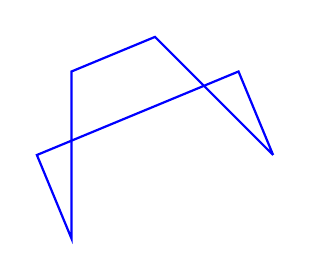
\begin{tikzpicture}[thick,scale=0.5]

	\coordinate (a) at (0:3);
	\coordinate (b) at (45:3); 
	\coordinate (c) at (90:3);
	\coordinate (d) at (135:3);
	\coordinate (e) at (180:3);
	\coordinate (f) at (225:3);
	\coordinate (g) at (270:3);
	\coordinate (h) at (315:3);

	\draw[blue] (a) -- (b) -- (e) -- (f) -- (d) -- (c) -- (a); 
	\draw (a) node {};
	\draw (b) node {};
	\draw (c) node {};
	\draw (d) node {};
	\draw (e) node {};
	\draw (f) node {};
	
\end{tikzpicture}
\hspace{2cm}
		\caption{A graph and the induced RGB graph.}
		\label{rgb}
	\end{center}
	\end{figure}

\subsection{Line Graphs}

 Proximity colorings and $RGB$ graphs become useful to connected matching problems when we consider {\it line graphs}\index{Line graph}.  The line graph of a graph $G$ (denoted $L(G)$) is a graph whose vertex set is the edge set of $G$ and vertices in $L(G)$ are adjacent if and only if the corresponding edges in $G$ share an endpoint. A simple example of a line graph is exhibited in Figure \ref{linegraph}.  
\begin{figure}

	\begin{center}
		\begin{tikzpicture}[thick,scale=0.5]

	\coordinate (a1) at (90:3);
	\coordinate (a2) at (-25:3); 
	\coordinate (a3) at (-155:3);
	\coordinate (a4) at (-90:3);
	\coordinate (a5) at (0:0);

	\draw (a5)-- node [lblvertex] {a}(a1);
	\draw (a5)-- node [lblvertex] {b}(a2);
	\draw (a5)-- node [lblvertex] {c}(a3);
	\draw (a5)-- node [lblvertex] {d}(a4);
	\draw (a3)-- node [lblvertex] {e}(a4);
	\draw (a2)-- node [lblvertex] {f}(a4);

	\draw (a1) node {};
	\draw (a2) node {};
	\draw (a3) node {};
	\draw (a4) node {};
	\draw (a5) node {};
	%\draw (a1) node[lblvertex] {a};
	%\draw (a2) node[lblvertex] {b};  
	
\end{tikzpicture}
\hspace{2cm}
		\begin{tikzpicture}[thick,scale=0.5]

	\coordinate (a) at (90:2.5);
	\coordinate (b) at (25:2.5); 
	\coordinate (c) at (0:0);
	\coordinate (d) at (155:2.5);
	\coordinate (e) at (-55:3);
	\coordinate (f) at (-125:3);

	\draw (a)--(b);
	\draw (b)--(c);
	\draw (c)--(d);
	\draw (d)--(a);
	\draw (a)--(c);
	\draw (c)--(d);
	\draw (b)--(e);
	\draw (e)--(c);
	\draw (d)--(f);
	\draw (f)--(c);
	\draw (d)--(b);
	\draw (e)--(f);
	%\draw (f) arc {-125:-33:3};
	
	\draw (a) node [lblvertex]{a};
	\draw (b) node [lblvertex]{b};
	\draw (c) node [lblvertex]{d};
	\draw (d) node [lblvertex]{c};
	\draw (e) node [lblvertex]{f};
	\draw (f) node [lblvertex]{e};
\end{tikzpicture}
\hspace{2cm}
		\caption{A graph and its line graph.}
		\label{linegraph}
	\end{center}
	\end{figure}

\begin{prop}
Connected matchings in a graph $G$ correspond to green cliques in the RGB graph induced by $L(G)$.  
\end{prop} 

\begin{proof}
	Incident edges of $G$ correspond to adjacent vertices in $L(G)$.  If we have a pair of edges $e, f \in E(G)$ that are disjoint and neighborly, then there is some edge $g \in E(G)$ between an endpoint of $e$ and an endpoint of $f$.  Hence, $eg, fg \in E(L(G))$ and $ef \notin E(L(G))$.  This means that $d_{L(G)}(e,f) = 2$, and $ef$ is green in the RGB graph induced by $L(G)$, as shown in Figure \ref{coresp}.  Since connected matchings are collections of pairwise non-incident and neighborly edges, the green cliques in the RGB graph induced by $L(G)$ correspond to connected matchings in $G$.  
\end{proof}
\begin{figure}
\begin{center}
\begin{tikzpicture}[thick,scale=0.5]

	\coordinate (a0) at (0:0);
	\coordinate (a1) at (180:1);
	\coordinate (a3) at (-109:3);
	\coordinate (a2) at (0:1);
	\coordinate (a4) at (-71:3);
	\coordinate (b1) at (150:3);
	\coordinate (b2) at (30:3);

	\draw (a0)-- node[lblvertex] {a}(a3);
	\draw (a0)-- node[lblvertex] {b}(a4);
	\draw (b1)[blue]--(b2);
	\draw (a0) node {};	
	%\draw (a1) node {};
	%\draw (a2) node {};
	\draw (a3) node {};
	\draw (a4) node {};
	\draw (b1) node[lblvertex, draw = blue] {a};
	\draw (b2) node[lblvertex, draw = blue] {b};
\end{tikzpicture}
\hspace{1cm}
\begin{tikzpicture}[thick,scale=0.5]

	\coordinate (a0) at (0:0);
	\coordinate (a1) at (180:1);
	\coordinate (a3) at (-109:3);
	\coordinate (a2) at (0:1);
	\coordinate (a4) at (-71:3);
	\coordinate (b1) at (150:3);
	\coordinate (b2) at (30:3);

	\draw (a1)-- node[lblvertex] {a}(a3);
	\draw (a2)-- node[lblvertex] {b}(a4);
	\draw (a1)--(a4);
	\draw (b1)[green]--(b2);
	%\draw (a0) node {};	
	\draw (a1) node {};
	\draw (a2) node {};
	\draw (a3) node {};
	\draw (a4) node {};
	\draw (b1) node [lblvertex, draw = green]{a};
	\draw (b2) node [lblvertex, draw = green]{b};
\end{tikzpicture}
\hspace{1cm}
\begin{tikzpicture}[thick,scale=0.5]

	\coordinate (a0) at (0:0);
	\coordinate (a1) at (180:1);
	\coordinate (a3) at (-109:3);
	\coordinate (a2) at (0:1);
	\coordinate (a4) at (-71:3);
	\coordinate (b1) at (150:3);
	\coordinate (b2) at (30:3);

	\draw (a1)-- node[lblvertex] {a}(a3);
	\draw (a2)-- node[lblvertex] {b}(a4);
	%\draw (a1)--(a4);
	\draw (b1)[red]--(b2);
	%\draw (a0) node {};	
	\draw (a1) node {};
	\draw (a2) node {};
	\draw (a3) node {};
	\draw (a4) node {};
	\draw (b1) node[lblvertex, draw = red] {a};
	\draw (b2) node[lblvertex, draw = red] {b};
\end{tikzpicture}

\label{coresp}
\caption{Correspondence between pairs of edges in $G$ and the RGB edges of $L(G)$.}
\end{center}
\end{figure}
Predictably, some complexity results on connected matching problems essentially rest on clique problems in RGB graphs of line graphs.  While clique problems are in general NP hard, there are special classes of graphs, such as perfect graphs, for which they can be solved efficiently.  We will see that some graphs retain this quality in the green graph of their line graph.
 
	%Introduction
	\chapter{THE EXTREMAL PROBLEM}


	Most of the work that has been done on connected matchings concerns the minimum size of a largest connected matching in a graph with certain properties.  This is the {\it extremal} problem of connected matchings.  In particular, how many vertices must a member of a certain class of graphs have before the existence of a connected matching of a certain size is guaranteed?  In this chapter we discuss a connection between a certain special case of Hadwiger's conjecture and the extremal problem of connected matchings.

\section{Extremal problems}

	 Extremal graph theory\index{Extremal graph theory} is concerned with finding the maximum or minimum (by a variety of measures) graphs that have a certain property.  Typically, an extremal problem asks ``How many edges must be present in a graph with $n$ vertices to ensure $X$'', or ``How many vertices must a graph with property $P$ have to ensure $X$''.  The iconic example of an extremal problem, one which we use in Section 3.2.1, is the problem of edges and cliques.  How many edges must a graph on $n$ vertices have to ensure the existence of a clique of size $k$?
The answer is due to T\'uran in 1941.  T\'uran's answer \cite{turan} explicitly constructed the extremal graph, that is, the graph on $n$ vertices with no $k$-clique and the maximum number of edges.  Let $T(n,r)$ be the graph on $n$ vertices constructed by dividing the vertices as evenly as possible into $r$ parts and adding all edges among the parts.  This is the {\it complete balanced $r$-partite graph} on $n$ vertices, also called a {\it T\'uran graph}.\index{T\'uran graph}
\begin{theorem}
	The $n$ vertex graph with no complete subgraph on $r$ vertices and the maximum number of edges is $T(n, r-1)$.
\end{theorem}
Many proofs of this theorem can be found in various graph theory texts, see \cite{PFTB} for several interesting proofs.

\section{A special case of Hadwiger's conjecture}

%\item Restricted versions of HC
	In Chapter 1 we discussed some partial results on Hadwiger's conjecture, primarily for the special cases arising from restricting the chromatic number.  Now we turn our attention to a different sort of special case.  A proper vertex coloring can be thought of as a partitioning of the vertex set into independent sets.  This gives us an easy lower bound on the chromatic number in terms of the size of a largest independent set.  The least number of colors needed would be realized when all color classes are the same size, so $\chi(G) \geq n/\alpha(G)$.  This leads to the following weakening of Hadwiger's conjecture.
\bconj{[Weaker version of Hadwiger's conjecture] For all graphs $G$, 
\[\eta(G) \geq \frac{n}{\alpha(G)}.\]}
At the present time, this conjecture is open for any particular value of $\alpha$.  However, it was recently shown by Fradkin \cite{fradkin} to hold for claw-free graphs with $\alpha \geq 3$. 
An examination of this problem by Duchet and Meyniel \cite{DandM} yielded the following bound.
\begin{theorem}
	For any graph $G$, 
\[\eta(G) \geq \frac{n}{2\alpha(G) -1}\]\label{dm}
\end{theorem}
This is turn was improved by Kawarabayashi et. al  \cite{Kawa} for almost all values of $\alpha$
\begin{theorem}
	For any graph $G$ on $n$ vertices with $\alpha(G) \geq 3$
\[\eta(G) \geq \frac{n(4\alpha(G)-2)}{(4\alpha(G)-3)(2\alpha(G)-1)}\]
\end{theorem}
The first improvement by an absolute constant factor comes from Fox \cite{fox} who shows that 
\begin{theorem}
	Let $c = \frac{29-\sqrt{813}}{28}$.  Then for any graph $G$,
\[\eta(G) \geq \frac{n}{(2-c)\alpha}\]\label{fox}
\end{theorem}
The specific case of $\alpha(G) = 2$ has attracted much attention.  Plummer, Stiebitz and Toft gave this case a thorough treatment in \cite{PST}.  Despite many partial and tangential results on this case, the bound in Theorem \ref{dm} is still the best known for $\alpha = 2$ (Note that for small values of $\alpha$, the bound in Theorem \ref{dm} is better than the bound in Theorem \ref{fox}).  In addition to their work on Hadwiger's conjecture, Plummer et. al introduce the  idea of a connected matching.  This led to the following extended conjecture.
\begin{conj}[PST extension of Hadwiger's conjecture] Every graph $G$ with $\alpha(G) = 2$ and $n$ vertices has a connected matching $M$ such that the contractions of the edges in $M$ to $|M|$ single vertices result in a graph containing $K_{\lceil n/c \rceil} $ 
\end{conj}
This was also conjectured by Seymour and is sometimes referred to as {\it Seymour's strengthening of Hadwiger's conjecture.}  Plummer, Stiebitz and Toft prove this conjecture for all inflations\footnote{An {\it inflation} of a graph is obtained by replacing some vertices with complete graphs of any size all of whose vertices are adjacent to the neighbors of the replaced vertex.} of graphs with independence number 2 and fewer than 12 vertices, as well as inflations of an infinite family of $\alpha = 2$ graphs.

\section{Connected matchings in graphs with $\alpha = 2$}

The strengthened version of Hadwiger's conjecture for graphs with independence number 2 placed connected matchings front and center.  Seymour is credited with presenting the problem of improving the bound of Duchet and Meyniel in the case of independence number 2.
\bconj{There exists $\epsilon > 0$ so that every graph $G$ with $n$ vertices and $\alpha(G) = 2$ contains $K_{\lceil(\frac{1}{3}+\epsilon)\rceil n}$ as a minor.\label{seym}}
One of the results of Kawarabayashi et. al in \cite{Kawa} effectively reduces this problem to an extremal problems on connected matchings.
\begin{theorem} If a graph $G$ on $n$ vertices with $\alpha(G) \leq 2$ contains a connected matching of size greater than or equal to $kn>0$, then $G$ has $K_{\lceil (n/3)(1+k/3)\rceil}$ as a minor.

Conversely, if $G$ has $K_{\lceil cn\rceil}$ as a minor for $c> \frac{1}{3}$, then $G$ contains a connected matching of size at least $(3c-1)n/4 -\frac{1}{2}$.\label{ramsey_flavor}
\end{theorem}
Thus, if there is some $k$ for which {\it every} graph with independence number two on $n$ vertices has a connected matching of size $kn$, then Conjecture \ref{seym} must be true.  Gy\'arf\'as, F\"uredi, and Simonyi presented this extremal conjecture explicitly in  \cite{GFS}
\bconj{There exists some constant $c$ such that every graph $G$ with $n$ vertices and $\alpha(G) = 2$ has a connected matching of size $cn$.\label{GFSconj}}
Furthermore, they conjecture on the value of the constant $c$
\bconj{Every graph $G$ with $4t-1$ vertices and $\alpha(G) = 2$ has a connected matching of size $t$.\label{GFSconj2}}
They prove this for values of $t$ up to 17, and show that it is sharp by exhibiting the example of $G$ consisting of two disjoint and disconnected cliques.

Another result found in \cite{PST} is that if $H$ is a 4-vertex graph with $\alpha(H) \leq 2$, and $G$ is an $n$ vertex graph with $\alpha(G) =2$ and no copy of $H$ as an induced subgraph, then $G$ has $K_{\lceil n/2 \rceil}$ as a minor.  Kriesell has recently \cite{Kries_1} improved this result by adding the 5 vertex graphs to this list.
\begin{figure}
	\begin{center}
	\begin{tikzpicture}[thick,scale=0.5]

	\coordinate (a) at (30:2.5);
	\coordinate (b) at (-30:2.5); 
	\coordinate (c) at (0:0);
	\coordinate (d) at (150:2.5);
	\coordinate (e) at (-150:2.5);
	%\coordinate (f) at (-125:3);

	\draw (c)--(b);
	\draw (c)--(a);
	\draw (c)--(d);
	\draw (c)--(e);
	\draw (b)--(a);
	\draw (d)--(e);
	
	\draw (a) node {};
	\draw (b) node {};
	\draw (c) node {};
	\draw (d) node {};
	\draw (e) node {};
	%\draw (f) node {};
	\draw (-90:4) node[words] {$B$};
	%\draw (-90:5) node[words] {but not a connected matching};
\end{tikzpicture}
\hspace{1.5cm}
	\begin{tikzpicture}[thick,scale=0.5]

	\coordinate (a) at (0:2.5);
	\coordinate (b) at (0:5); 
	\coordinate (c) at (0:0);
	\coordinate (d) at (150:2.5);
	\coordinate (e) at (-150:2.5);
	%\coordinate (f) at (-125:3);

	%\draw (a)--(b);
	\draw (c)--(a);
	\draw (c)--(d);
	\draw (c)--(e);
	\draw (b)--(a);
	\draw (d)--(e);
	
	\draw (a) node {};
	\draw (b) node {};
	\draw (c) node {};
	\draw (d) node {};
	\draw (e) node {};
	%\draw (f) node {};
	\draw (-90:4) node[words] {$B^-$};
	%\draw (-90:5) node[words] {but not a connected matching};
\end{tikzpicture}

	\end{center}
	\caption{The graphs $B$ and $B^-$ referred to in Theorem \ref{Kriesell2}.}
	\label{B_B}
\end{figure}
\begin{theorem}
	Let $H$ be any graph with $\alpha(H) \leq 2$ on at most 5 vertices.  Then every $\{\kfree, H\}$-free graph on $n$ vertices has a collection of $\lceil n/2 \rceil$ pairwise adjacent edges and vertices.
	\end{theorem}
From this and the second part of theorem  \ref{ramsey_flavor} we conclude that every $\{\kfree, H\}$-free graph on $n$ vertices has a connected matching of size $\lfloor \frac{n}{8} \rfloor$. However when $H = \overline{K_{2,3}}$, Kriesell has found that we can say even more.
\begin{theorem}
	Every connected, $\{\kfree, \overline{K_{2,3}}\}$-free graph on $n$ vertices nonisomorphic to $B$ or $B^-$ in Figure \ref{B_B} has a connected dominating matching of size $\lfloor \frac{n}{2} \rfloor$.\label{Kriesell2}
\end{theorem}


 	%Extremal problems and conjectures
	\chapter{The GFS conjecture}

In this chapter, we examine the progress that has been made on conjecture REF, and present some new partial results.  We will see that for $\kfree$-free graphs with very large cliques, as well as sufficiently large $\kfree$-graphs with only the smallest possible cliques, the conjecture holds.

\section{The properties of a counterexample}

Gy\'{a}rf\'{a}s, F\"{u}redi and Simonyi prove their conjecture for graphs up to 67 vertices.  In so doing, they implicitly introduce an important lemma concerning the relationship between cliques and connected matchings.  

\blem{[GFS] Let $0<c<1/4$.  If $G$ is a $\kfree$-free graph with $\omega(G) \geq cn$, then $G$ has a $\lfloor cn\rfloor$-connected matching.
\label{spider}}
\begin{proof}
	Let $S$ be a set of $\lceil cn\rceil$ vertices inducing a clique.  For any subset of $S'\subseteq S$, the intersection $\displaystyle I = \bigcap_{s\in S'} \{v \in V(G): sv \notin E(G)\}$ induces a clique.  If for any $S'\subseteq S$, $|I| > n/2$, then there is a $n/2$-connected matching in the clique induced by $I$.  Otherwise, 
\begin{align*}
|N(S')| &= n- |S'| - |I|\\
	&\geq n - |S'| - \frac{n}{2}\\
	&\geq \frac{n}{4} \\
	&> |S'| 
\end{align*} for all $S'\subseteq S$.  Hence, by Hall's condition (see {\it e.g.}, \cite{West}),  a matching from the vertices of $S$ to the vertices of $V(G)-S$.  This matching must be connected, since $S$ induces a clique.
\end{proof}

We might evocatively call this the ``spider lemma'' as it exhibits a connected matching with a ``head'' (the clique) and many ``legs'' (the matching with one side inducing the clique).  Using the spider lemma, we can deduce some structural qualities that a counterexample to conjecture REF must possess.  Chief among these will be connectivity, as disconnected vertex sets in $\kfree$-free graphs induce cliques.  First, we will make explicit the relationship between the GFS conjecture and Seymour's strengthening of Hadwiger's conjecture (hereafter SSH).  The following proposition shows that SSH implies the GFS conjecture.  

\bprop{If SSH holds for a $K_3$-free graph $G$ with $n$ vertices, then $\nu_c(G) \geq n/4$.}

\begin{proof}
Let $\mathcal{M}$ be the collection of branch sets of an $n/2$ SSH-minor of $G$. Let $M_1$ be the collection of elements of $\mathcal{M}$ consisting of single vertices and $M_2$ the collection of elements of $\mathcal{M}$ consisting of edges.  Obviously $M_2$  is a connected matching.  Furthermore, any matching of the clique induced by $M_1$ forms a connected matching that extends the connected matching formed by $M_2$.  Hence, 
\[\nu_c(G) \geq \lfloor\frac{|M1|}{2}\rfloor + |M2| \geq \lfloor\frac{|M1 | + |M2 |}{2}\rfloor = \lfloor n/4\rfloor\]
\end{proof}

In Lemma 2.1 of \cite{Blas}, Blasiak shows that any $\kfree$-free graph with connectivity less
than $n/2$ satisfies SSH. We can show the following for higher connectivity.  

\blem{ If G is a $\kfree$-free graph on $n$ vertices, then  $\nu_c(G) \geq \frac{n-\kappa(G)}{4}$. If $\kappa(G) \geq n/2$, then $\nu_c(G) \geq
n -\kappa(G)$. }% Furthermore, if $n/4 < \kappa(G) < n/2$, then $\nu_c(G) \geq \kappa(G)$ and if $\kappa(G) < n/4$ then $\nu_c(G) \geq n/2 - \kappa(G)$}

\begin{proof} Let $G$ be a $\kfree$-free graph on $n$ vertices. A minimum cut set separates two cliques, at least one of which has at least  $\frac{n-\kappa(G)}{2}$ vertices.  Any matching in this clique is connected, so we can find a  $\frac{n-\kappa(G)}{4}$ connected matching. 

The proof of the second claim follows the strategy of Lemma 2.1 of \cite{Blas}. 
%
From this point on, we will assume that $\kappa(G) \geq n/2$.
%
Let $S$ be a minimum cut set of $G$. 
%
Then let $L$, $R$ be a partition of $V(G)-S$ so that $L$ and $R$ do not touch. 
%
Since $G$ is $\kfree$-free, $L$ and $R$ are cliques, and every vertex of $S$ is complete to $L$ or complete to $R$. 
%
Let $S_L$ be the set of vertices complete to $L$ and $S_R$ be the set of vertices complete to $R$. 
%
We claim that between any $A \subseteq S_L$ with $|A| \leq |R|$ and $R$ ($S_R$ and $L$ resp.) there is a matching that saturates $A$. 
%
Suppose there is no matching from $R$ that saturates $A$. 
%
Hall’s condition then implies that there is a subset $T$ of $A$ such that $|N(T) \cap R| < |T |$. 
%
But then $(S -T) \cup (N(T)\cap R)$ is a cut set separating $L \cup T$ and $R - N (T)$. 
%
This set is smaller than $S$, yielding a contradiction.

Let $M$ be the largest possible matching obtained with edges between $S_L$ and $R$ (temporarily dubbed {\it type 1 edges}) and edges between $S_R$ and $L$ ({\it type 2 edges}). 
%
This matching is connected.
%
To see this, note that both types of edge form ``spiders'' as $R$ and $L$ are cliques.
%
Furthermore, without loss of generality, the $S_L$ ends of the type 1 edges are complete to $L$, and hence adjacent to an endpoint of every type 2 edge.
%

If both $|R| \leq |S_L|$ and $|L| \leq |S_R|$ (and $\kappa(G) \geq n/2$) , then we can find $T_L \subseteq S_L$ and $T_R \subseteq S_R$ so that $T_L$ and $T_R$ are disjoint, $|T_R| = |L|$, and $|T_L| = |R|$. 
%
Thus by the above claim we can construct a connected matching saturating $V(G)-S$.  
%

Now suppose, without loss of generality, that $|R| > S_L$.
%
Note that it cannot also be the case that $|L| > S_R$, as $S \geq n/2$ and $S \subseteq S_L \cup S_R$.
%
Let $R^u$ denote the set of vertices of $R$ unmatched by $M$.
%
Since $|S| \geq n/2$, we can assume that we have matched all the vertices of $S_L$ to vertices in $R$.  
%
This also means that there are at least $|R^u|$ unmatched vertices of $S_R$ (denoted $S_R^u$ ).
%
 Augment $M$ with any matching from the biclique between $R^u$ and $S_R^u$ saturating $R^u$ to yield $M'$ . 
%
These new edges are mutually connected, and connected to any type 1 or type 2 edges via edges of $R$ in the case of type 1, or edges from $S_R$ to $R$ in the case of type 2. 
%
Now $M'$ is a connected matching saturating $R \cup L$, and $|R \cup L| = n- \kappa(G)$.
\end{proof}

This lemma, together with the spider lemma, allow us to collect the properties of what we might call a ``large-clique'' counterexample to the GFS conjecture.   The following must hold in order that the largest clique is not so large that we may apply the spider lemma to find a large connected matching.
  
\bprop{
	If $G_c$ is a counterexample to conjecture \cite{GFS} with the constant $c$, then the following conditions must hold
	\begin{enumerate}
		\item $\omega(G_c) < cn$.
		\item $\delta(G_c) \geq (1 - c )n$.
		\item $G_c$ has diameter 2.
		\item  $G_c$ is $(1 - c)n$-connected.
	\end{enumerate}
}

Items 1 and 4 come directly from the two lemmas we have just presented.  That the collection of non-neighbors of a vertex in a $\kfree$-free graph form a clique leads to item 2.  Applying the pigeonhole principle to item 2 we see that every pair of vertices share a neighbor, so $G_c$ has diameter 2.  Thinking inductively, we can add to our list by considering a {\it vertex-minimal} counterexample.
\bprop{If $G_c$ is a vertex-minimal counterexample to \cite{GFS} with the constant $c$, then $G_c$ has no edge dominating $n-1/c$ vertices.}
If $G$ has an edge domminating $n-1/c$ vertices, then by an induction hypothesis we can assume it dominates a $\lfloor cn\rfloor-1$ connected matching and extends it by one.   

Taken altogether, the results of this section show that a counterexample to \ref{GFS} must be highly connected, yet lack large cliques.  In the next section we will eliminate from consideration a class of $\kfree$-free graphs that are highly connected and possess only the {\it smallest} possible cliques. (BLASIAK QUOTE ABOUT THE ``INTERESTING CASES'')

\section{Graphs with no large cliques}

In \cite{MR1369063}, Kim famously proved that the magnitude of the Ramsey number $R(3,k)$ is $\Theta(k^2/\log k)$.
%
This means that for any fixed $c$ there are $\kfree$-free graphs whose largest cliques are on the order $\sqrt{n\log n}$. 
%
These graphs are also very highly connected, so the results of the previous section are of no help.
%
CITE DEF The so-called \textit{Ramsey graphs}...
%
In this section, we will show the GFS conjecture holds for sufficiently large Ramsey graphs, witha value of $c$ arbitrarily close to $1/4$.
%
We will also discuss a natural random $\kfree$-free graph model which almost certainly satisfies the GFS conjecture. 

\begin{theorem}
Let $c < 1/4$ be a constant.  For any constant $b$ and sufficently large $n$, every $\overline{K_3}$-free graph $G$ on $n$ vertices with $\omega(G) < b\sqrt{n\log n}$ has a $cn$-connected matching.
\label{sm_cli}
\end{theorem}

First, we will prove a lemma that will place a bound on the number of pairs of separable edges in a $\kfree$-graph with a given clique number.  In order to simplify the notation in the proof, we will work on the complementary notion of {\it cycles of four vertices} in {\it $K_3$-free} graphs with a given {\it independence} number.  

\begin{lem}
For every pair of positive constants $\epsilon, d$ there is $n_{\epsilon, d}$ such that every triangle-free graph $G$ with $n > n_{\epsilon, d}$ vertices and $\alpha(G) < d\sqrt{n\log n}$ has fewer than $\epsilon n^3$ copies of $C_4$.
\end{lem}
\begin{proof}
Fix $\epsilon, d> 0$ and let $G$ be a triangle free graph on $n$ vertices with $\alpha(G) < d\sqrt{n\log n}$.  
%
Let $X_{C_4}$ be the number of copies of $C_4$ in $G$.  
%
Then
%
\begin{equation}
X_{C_4} = \frac{1}{2}\sum_{\{u,v\}\notin E(G)} {|N(u) \cap N(v)| \choose 2} 
\label{c4counteq}
\end{equation}
%
\begin{figure}
	\begin{center}
		\begin{tikzpicture}[thick,scale=0.6]

\draw (-4,4) node[lblvertex]{x}
	edge[dashed] (4,4)
	edge[] (-.8,-1.2)
	edge[] (.8, -2.3);
	
\draw(4,4) node[lblvertex]{y}
	edge[] (-.8,-1.2)
	edge[] (.8, -2.3); 
	
\draw[fill = red, opacity = 0.25](-2,-2) ellipse (4 cm  and 2.5 cm);
\draw[fill = blue, opacity = 0.25](2,-2) ellipse (4 cm and 2.5 cm);

\draw (-3.8,-2) node[words]{$N(x)$};
\draw (3.8,-2) node[words]{$N(y)$};

\draw (-.8,-1.2) node[]{}
	edge[dashed] (.8,-2.3);
\draw (.8,-2.3) node[]{};

\end{tikzpicture}	
	\end{center}
	\label{c4count}
	\caption{Illustration of the count from Eq. \ref{c4counteq}}
\end{figure}
%
For each nonadjacent vertex pair $\{u,v\}$, we count the number of distinct pairs of vertices in the intersection of the neighborhoods of $u$ and $v$.  This counts each $C_4$ twice, so we divide by two. 
%
Fix $\epsilon_1 < \sqrt{8\epsilon}$.

\noindent\textit{Claim. For sufficiently large $n$, fewer than $n^2(\log n)^{-2}$ pairs of vertices $u,v$ have neighborhood intersection larger than $\epsilon_1\sqrt{n}$.}

Suppose the contrary is true, and there are more than $n^2(\log n)^{-2}$ pairs $u,v$ so that $|N(u)\cap N(v)| \geq \epsilon_1\sqrt{n}$.
%
When we count the total number of vertices in these intersections, the count is at least $\epsilon_1n^{5/2}(\log n)^{-2}$, meaning some vertex is counted at least $\epsilon_1n^{3/2}(\log n)^{-2}$ times.  However, $\Delta(G) \leq \alpha(G) < d\sqrt{n\log n}$, so each vertex is in at most \[{d\sqrt{n\log n}\choose 2 } < \frac{d^2}{2}n\log n\] neighborhood intersections.  Thus, for sufficiently large $n$,  the claim holds.

Now we can bound $X_{C_4}$.  We will overestimate by supposing that there are precisely $n^2(\log n)^{-2}$ pairs of vertices with the largest possible vertex intersection, and the remainder have neighborhood intersection of size $\epsilon_1\sqrt{n}$.
\begin{equation}X_{C_4} < \frac{1}{2}\left[\frac{n^2}{(\log n)^2}{d\sqrt{n\log n}\choose 2}+ \left(|E(\overline{G})|- \frac{n^2}{(\log n)^2}\right){\epsilon_1\sqrt{n}\choose 2}\right]
\end{equation}
Evaluating the right hand side asymptotically we have	
\begin{equation}
\sim \frac{\epsilon_1^2-2\epsilon_1}{8}n^3 
\end{equation}
This is strictly greater than $\epsilon n^3$, so for sufficiently large $n$, the desired bound on $X_{C_4}$ holds.
\end{proof}
 
Now we can prove theorem \ref{sm_cli}.  We will use the language of RGB proximity colorings introduced in chapter 1. 

\begin{proof}[Proof (of Theorem \ref{sm_cli})]
Fix constants $d$ and $c < 1/4$, and let $G$ be a $\overline{K_3}$-free graph with $n$ vertices, $m$ edges, and $\omega(G) < b\sqrt{n\log n}$.  
%
Consider the $RGB$ graph $\mathcal{G}$ induced by $L(G)$ (recalling that green $k$-cliques correspond to $k$-connected matchings in $G$ and red edges correspond to induced $\overline{C_4}$s in $G$).
%
If $R, G,$ and $B$ denote the number of red, green and blue edges respectively, we would like to show that 
\begin{equation}
G = {m\choose 2} - R - B \geq {m\choose 2} - cn{m/cn\choose 2}
\end{equation} equivalently
\begin{equation}
	R + B \leq cn{m/cn\choose 2}\label{goal}
\end{equation}
guaranteeing by T\'{u}ran's theorem (see, \textit{e.g.}, \cite{dwest}) a green clique on $cn$ vertices in $\mathcal{G}$, and a $cn$-connected matching in $G$.

We obtain a crude upper bound on $B$ by taking the number of edges in the line graph of $K_n$.
\begin{equation}
	B < \frac{n^3}{2} - \frac{3n^2}{2} + n
\end{equation}
We can bound $R$ using Lemma 1.  For any $\epsilon > 0$ and sufficiently large $n$, 
\begin{equation}
R < \epsilon n^3\
\end{equation}
Thus for sufficiently large $n$,
\begin{equation}
	B+R < \frac{n^3}{2} + \epsilon n^3
\end{equation}
We compare this with the right hand side of (\ref{goal})
\begin{eqnarray}
	cn{m/cn\choose 2} =&\displaystyle \frac{cn}{2}\left(\frac{m^2}{c^2n^2} - \frac{m}{cn}\right)\\
	=& \displaystyle \frac{1}{2c}m^2n^{-1} - \frac{m}{2}\\
	\sim&   \displaystyle \frac{n^3}{8c}
\end{eqnarray}
Since $c < 1/4$, and we can take $\epsilon < \frac{1-4c}{8c}$, for sufficiently large $n$ (\ref{goal}) holds and $G$ has a $cn$-connected matching.
\end{proof}

The \textit{triangle free process} is a method of stochastically constructing maximal triangle free graphs.  Let $G_0$ be the empty graph on $n$ vertices and let $O_i$ be the set of edges of $K_n- G_i$ that will not create a triangle when added to $G_i$.  Then for each $G_i$, construct $G_{i+1}$ by adding an edge chosen uniformly at random from $O_i$ until some step $k$ at which $O_k$ is empty.  The complementary version of this process is a natural source of $\overline{K_3}$-free graphs.  It is worth noting, therefore, that Bohman has shown in CITE that the triangle free process asymptotically almost surely produces graphs which satisfy the hypotheses of Theorem \ref{sm_cli}.  This falls somewhat short of a proof that the GFS conjecture holds for almost all $\kfree$-free graphs because the triangle-free process does not produce a uniform distribution. ADD NOTE ABOUT APPEARANCE OF SUBGRAPHS

In conclusion, we can see that in $\kfree$-free graphs that are highly ``spread-out'' (Theorem \ref{sm_cli}) and in ones that are ``bunched-up'' (spider lemma) the GFS conjecture succeeds.   It remains to be seen if further work in tuning and sharpening these techniques can close the gap, if new approaches are needed, or if indeed there lurks a counterexample somewhere in the middle ground.

	%The GFS conjecture%
	\chapter{Computing $\nu_c(G)$}

Given a graph $G$, we would like to be able to calculate the connected matching number $\nu _c(G)$.  
%
The general problem of calculating the connected matching number was shown to be NP-hard by Plummer, Stiebitz and Toft CITE.  
%
\begin{framed}
	\noindent\textbf{k-Connected Matching}
	\vskip 0.5cm
	\noindent Input: Graph $G$, positive integer $k$
	
	\noindent Question: Is there a connected matching in $G$ of size $k$?
\end{framed}
In this chapter, we consider the complexity of finding the largest connected matching in members of some special families of graphs.

\section{Known results}

In CITE, Kathie Cameron shows that the maximum connected matching problem is solvable in polynomial time for {\it chordal} graphs.   
%
To do this, we first think of connected matchings as matchings contained in {\it neighborly} sets of edges.  
%
Neighborly sets of edges from a graph $G$ correspond to cliques in the square of the line graph of $G$, $L(G)^2$.  
%
It then follows that if $L(G)^2$ has $M$ maximal cliques, then finding the maximum connected matching in $G$ can be done by solving $M$ maximum matching problems.  
%
Hence, we can state the following general result from which the result on chordal graphs follows.
%
\bthm{If $\mathcal{P}$ is a class of graphs such that for any $G \in \mathcal{P}$ with $n$ vertices, the number of maximal cliques in $L(G)^2$ is less than $f(n)$ where $f$ is a polynomial, then the maximum connected matching problem can be solved in polynomial time for graphs from $\mathcal{P}$.}
%
One can show that the square of the line graph of a chordal graph is itself a chordal graph, and hence has a polynomial number of maximal cliques. SOME OTHER CLASSES ARE...
%

Conversely, Cameron also shows that the problem remains NP complete on 0-1 weighted bipartite graphs.  
%
It is not difficult to reduce this problem to the maximum clique problem on general graphs.  
%
We simply take any graph $H$ and replace each vertex $v$ with an edge $v_1$ and $v_2$.  This edge is given weight 1.  
%
Then if two vertices $u$ and $v$ are adjacent in $H$, we place an edge between $u_1$ and $v_2$ or $u_2$ and $v_1$.
%
These edges are given weight zero.
%  
Then the edges of positive weight in any connected matching in the resulting graph corresponds to a clique in $H$ and vice versa.
%
It is important to note that this reasoning will not extend to the unweighted bipartite graphs.  


\section{Chordal Bipartite Graphs}

To extend these results, we turn our attention to a relaxation of chordal graphs, the {\it weakly} chordal graphs. 
%
A weakly chordal graph is one in which every cycle of length five or greater has a chord.  
%
In particular, we will closely examine those weakly chordal graphs which are also bipartite.  
%
These graphs are known as {\it chordal bipartite} graphs.  
\begin{figure}
	\begin{center}
		
\begin{tikzpicture}[thick,scale=0.4]


\draw[ fill = red, opacity = 0.25] (0,0) circle (3);
\draw[ fill = blue, opacity = 0.25, thin] (3.5,0) circle (3);
\draw[ fill = red, opacity = 0.25] (0,0) circle (1.5);

\draw  (-4,4.5) node[words]{weakly chordal}
	edge [->, thin] (-1,2.9);

\draw  (-4,-4.5) node[words]{chordal}
	edge [->, thin] (-1.3,-0.9);

\draw (1,-4.5) node[words]{acyclic};
\draw node[words] (1,-4) {}
	edge [->, thin] (1,-.5);


\draw (6, -5.5) node[words]{chordal bipartite}
	edge[->, thin] (2,-.5);
\draw (5, 4.5) node[words]{bipartite}
	edge[->,thin] (4.5,2.85);

\end{tikzpicture}

	\end{center}
	\label{inclusion}
	\caption{Inclusion Diagram}
\end{figure}

An important characterization of chordal bipartite graphs is that any non-empty induced subgraph of a chordal bipartite graph contains a {\it bisimplicial edge}.  
%
An edge $uv$ is bisimplicial if the neighborhoods of the endpoints induce a complete bipartite graph.  
%
That is, for any $a\in N(u)$ and $b\in N(v)$, $ab$ is an edge of the graph.  
%
Bisimplicial edges equip the chordal bipartite graphs with an elimination ordering, i.e., upon removing a bisimplicial edge from a chordal bipartite graph, the resulting graph is still chordal bipartite.

\subsection{Inert bisimplicial edges}
If a graph is non-separable, then we can quickly compute the maximum connected matching using any maximum matching algorthim we choose.  
%
The following result of Golumbic is valuable when dealing with non-separable chordal bipartite graphs.
%
\bthm{[Golumbic, 1979] Let $H$ be a chordal bipartite graph.  If $H$ is separable, then it has at least two separable bisimplicial edges.}
%
We will see shortly that once we have identified a pair of bisimplicial edges, we can always remove one of them from the graph  
%

Let us say that an edge $e$ in a graph $G$  is {\it inert} if $\nu_c{G} = \nu_c(G-e)$.  
%
Bisimplicial edges in chordal bipartite graphs are inert unless the conditions in the following lemma are satisfied.
%
\blem{Let $G = (A, B; E)$ be chordal bipartite.  A bisimplicial edge $e = uv$ is inert unless
	\begin{enumerate}
 		\item $e$ is contained in every maximum connected matching.
		\item For any maximum connected matching $M$, every edge of $M$ has
 exactly one endpoint adjacent to an endpoint of $e$.
		\item For any maximum connected matching $M$, $N(e)$ is covered by M
	\end{enumerate}
}
%
\begin{figure}
	\begin{center}
	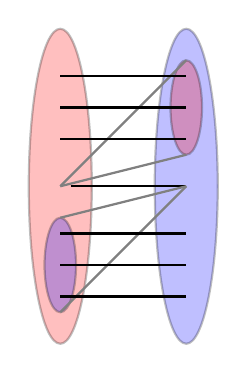
\begin{tikzpicture}[thick,scale=0.4]

\draw[fill = red, opacity = 0.25]  (-2,0) ellipse(1 and 5);
\draw [fill = blue, opacity = 0.25](-2,-2.5) ellipse (0.5 and 1.5);
\draw[fill = blue, opacity = 0.25] (2,0) ellipse (1 and 5);
\draw[fill = red, opacity = 0.25] (2,2.5) ellipse (0.5 and 1.5);
\draw (-2,0) node[]{}
	edge[] (2,0);
\draw (2,0) node[]{};

\draw[color = gray] (-2,0)--(2,4);
\draw[color = gray] (-2,0)--(2,1);
\draw[color = gray] (2,0)--(-2,-1);
\draw[color = gray] (2,0)--(-2,-4);

\draw (-2,3.5)--(2,3.5);
\draw (-2,2.5)--(2,2.5);
\draw (-2,1.5)--(2,1.5);
\draw (-2,-3.5)--(2,-3.5);
\draw (-2,-2.5)--(2,-2.5);
\draw (-2,-1.5)--(2,-1.5);
\end{tikzpicture}
	\end{center}
	\label{bisimp_pic}
	\caption{Picture of a non-inert bisimplicial edge.  Every maximum connected matching saturates the neighborhood of the edge with no connected matching edge left over.}
\end{figure}
%
\begin{proof}
Suppose we have a chordal bipartite graph $G = (A,B;E)$ that has a bisimplicial edge $e = uv$ with $u \in A$ and $v \in B$.  
%
To prove 1, we must show that removing $e$ does not reduce the size of a maximum connected matching that does not include $e$. 

In fact we can show more, to wit, that removing $e$ does not reduce the size of {\it any} connected matching that does not include $e$.  
%
Suppose we have a connected matching $M$.  
%
If $M$ does not cover $e$, then obviously removing $e$ has no effect on the size of $M$.  
%
Thus we have $f = uu'$ and $g = v'v$ included in $M$.  
%
The only way removing $e$ can reduce the size of $M$ is by disconnecting $f$ and $g$.  
%
However, since $e$ is bisimplicial, $u' \in N(u)$, and $v' \in N(v)$; the edge $u'v'$ must be present.  
%
Hence removing $e$ does not disconnect $f$ and $g$.
\begin{figure}
	\begin{center}
	\begin{tikzpicture}[thick,scale=0.8]

\draw (0, 4) node[words]{$M$};


\draw (1, 3) node[]{}
	edge[color = gray] (-1, 3);
\draw (-1, 3) node[]{};
\draw (1, 2) node[]{}
	edge[color = gray] (-1, 2);
\draw (-1, 2) node[]{};
\draw (1, 1) node[]{}
	edge[color = gray] (-1, 1);
\draw (-1, 1) node[]{};
\draw (1, 0) node[]{}
	edge[color = gray] (-1, 0);
\draw (-1, 0) node[]{};

\draw[color = red] (1,3) -- (-1,0);
\draw[color = green] (-1,3)--(1,0);
\draw[color = red] (0,1.5) node[lblvertex]{e};


\draw (0,-0.5) node[dot]{};
\draw (0,-0.8) node[dot]{};
\draw (0,-1.1) node[dot]{};

\draw (1, -1.6) node[]{}
	edge[color = gray] (-1, -1.6);
\draw (-1, -1.6) node[]{};
\end{tikzpicture}
	\end{center}
	\label{first_part}
	\caption{Illustration of proof of condition 1.}
\end{figure}
%
In proving 2, we choose a maximum connected matching $M$.  
%
By 1, we can assume that $e \in M$.  
%
Suppose now that $f = u''v''$ is another edge of $M$ and edges $g = uv''$ and $h = u''v$ are both present.  
%
We claim that we can remove $e$ and $f$ from $M$ and replace them with $g$ and $h$. 
%
 Let $d = u'''v'''$ be an edge of $M$.  
%
This edge $d$ must be connected to one of the two via an endpoint of $e$.  
%
Without loss of generality, suppose $d$ is connected to $g$ via $uv'''$.  
%
Now $v''' \in N(u)$ and $u'' \in N(v)$.  
%
Since $u$ is bisimplicial, $u''v'''$ is present and $d$ is connected to $h$ as well.
\begin{figure}
	\begin{center}
	\begin{tikzpicture}[thick,scale=0.8]

\draw (0, 4) node[words]{$M$};


\draw (1, 3) node[]{}
	edge[color = gray] (-1, 3);
\draw (-1, 3) node[]{};
\draw (1, 2) node[]{}
	edge[color = green] (-1, 2);
\draw (-1, 2) node[]{};
\draw (0,2) node[lblvertex]{e};
\draw (1, 1) node[]{}
	edge[color = gray] (-1, 1);
\draw (-1, 1) node[]{};
\draw (1, 0) node[]{}
	edge[color = green] (-1, 0);
\draw (0,0) node[lblvertex]{f};
\draw (-1, 0) node[]{};

\draw[color = blue] (1,2)--(-1,0);
\draw[color = blue] (-1,2)--(1,0);


\draw (0,-0.5) node[dot]{};
\draw (0,-0.8) node[dot]{};
\draw (0,-1.1) node[dot]{};

\draw (1, -1.6) node[]{}
	edge[color = gray] (-1, -1.6);
\draw (-1, -1.6) node[]{};
\end{tikzpicture}
	\end{center}
	\label{second_part}
	\caption{Illustration of proof of condition 2.}
\end{figure}
%
To prove 3, once again choose a maximum connected matching $M$.  
%
Suppose now that 3 does not hold, and there is (WLOG) an edge $f = ux$ such that $x$ is not covered by $M$.  
%
We claim that we can remove $e$ and replace it with $f$ in $M$.  We need only consider some $M$ edge $g$ that is not connected to $e$ via $u$.  
%
Then there is an endpoint $w$ of $g$ so that $w \in N(v)$.  
%
Clearly $x\in N(u)$, so $wx$ is present and $g$ is connected to $f$.
\begin{figure}
	\begin{center}
	\begin{tikzpicture}[thick,scale=0.8]

\draw (0, 4) node[words]{$M$};


\draw (1, 3) node[]{}
	edge[color = gray] (-1, 3);
\draw (-1, 3) node[]{};
\draw (1, 2) node[]{}
	edge[color = green] (-1, 2);
\draw (-1, 2) node[]{};
\draw (0,2) node[lblvertex]{e};
\draw (1, 1) node[]{}
	edge[color = gray] (-1, 1);
\draw (-1, 1) node[]{};
\draw (1, 0) node[]{}
	edge[] (-1, 0);
\draw (-1,0) node[]{};

\draw (2,0) node[]{}
	edge[color = blue] (-1,2);
\draw (1.5,0.3) node[lblvertex]{f};


\draw (0,-0.5) node[dot]{};
\draw (0,-0.8) node[dot]{};
\draw (0,-1.1) node[dot]{};

\draw (1, -1.6) node[]{}
	edge[color = gray] (-1, -1.6);
\draw (-1, -1.6) node[]{};
\end{tikzpicture}
	\end{center}
	\label{third_part}
	\caption{Illustration of proof of condition 3.}
\end{figure}
\end{proof} 

If we can quickly determine which bisimplicial edge of a separable pair is inert, then we can sequentially remove them until the resulting graph is no longer separable.  
%
In fact, this test essentially reduces the maximum connected matching problem to a {\it saturating } connected matching problem.  
%
If a bisimplicial edge is not inert, then Lemma REF shows that it must have connected matchings that cover the neighborhoods of each endpoint.  
%
If such a condition holds for both of a pair of separable bisimplicial edges, then we can simply remove the edge with fewer incident edges (or either one if the number of incident edges is the same).  
%
Going forward then, we can restrict our attention to the following smaller problem.  NEED TO CLARIFY THIS DISTINCTION
\begin{framed}\noindent\textbf{Saturating Connected Matching}
	\vskip 0.5cm
	\noindent Input: Bipartite graph $G = (A,B;E)$
	
	\noindent Question: Is there a connected matching in $G$ that saturates $A$?
\end{framed}
\subsection{Ordered connected matchings}

Connected matchings in chordal bipartite graphs have a special property.
%
We define an {\it ordered} connected matching as follows.
%  
\begin{mydef}[Ordered Connected Matching]
	Let $M = \{e_1, e_2, \ldots, e_k\}$ be a connected matching in a bipartite graph $G = (A,B; E)$ and label the endpoints of each $e_i$ by $a_i \: (\in A)$ and $b_i \: (\in B)$.  If there is an ordering $\sigma : M \rightarrow [k]$ so that 
	\begin{enumerate}
		\item $deg(a_i) \geq \sigma(e_i)$ for each $i\in [k]$ and 
		\item $N(a_l) \subseteq N(a_j)$ whenever $j \geq l$ for all $j,l \in [k]$
	\end{enumerate} 
then we say $M$ is an ordered connected matching
\end{mydef}
%
Note that if we find the appropriate sequence of vertices in $A$, there is neccessarily an appropriate sequence of vertices in $B$.  
%
\begin{figure}
	\begin{center}
	
\begin{tikzpicture}[thick,scale=1]

\draw[color = gray] (-1,2)--(1,1);
\draw[color = gray] (-1,1)--(1,0);
\draw[color = gray] (-1,0)--(1,2);

\draw (1, 2) node[]{}
	edge[color = black] (-1, 2);
\draw (-1, 2) node[]{};
\draw (1, 1) node[]{}
	edge[color = black] (-1, 1);
\draw (-1, 1) node[]{};
\draw (1, 0) node[]{}
	edge[color = black] (-1, 0);
\draw (-1, 0) node[]{};


\end{tikzpicture}
	\end{center}
	\label{c_6}
	\caption{A connected matching that is not an ordered connected matching.}
\end{figure}
%
Not every bipartite connected matching is an ordered connected matching, as we can see in figure \ref{c_6}. 
%
 However, it is worth noting that this example is a cycle on six vertices.  
%
Appropriately, we can prove the following.
%
\bthm{Every connected matching in a chordal bipartite graph is an ordered connected matching.}
\begin{proof}
%
We will show that any connected matching $M$ in a chordal bipartite graph $G = (A,B; E)$ has a vertex $a \in A$ so that $a$ is covered by $M$ and $a$ is adjacent to the $B$-endpoints of every edge of $M$.  
%
We will say that such a vertex {\it dominates} $M$.  
%
If this is true, we can find the proper ordering of $M$ by sequentially removing the $M$-edge covering a dominating edge and working on the smaller connected matching that remains.

We will proceed by induction on the size $n$ of the connected matching.  
%
Small cases of $n = 1,2$ are trivial, and the case of $n=3$ is easily checked.  
%
Now suppose that every chordal bipartite connected matching of up to $n-1$ edges has a dominating vertex and let $M$ be a connected matching of size $n$ in a chordal bipartite graph $G = (A,B;E)$.  
%
Let $H$ be the subgraph of $G$ induced by vertices covered by $M$.
%
Applying lemma REF, we can remove any bisimplicial edges of $H$ that are not contained in $M$ without reducing the size of $M$.  
%
Neither does this introduce any new dominating vertices.  
%
Remove these edges until all remaining bisimplicial edges are contained in $M$.  

The resulting graph is chordal bipartite, so there exists a bisimplicial edge $ab \in M$, with $a \in A$ and $b \in B$.  
%
If $a$ is not a dominating vertex, then consider $M_b$, the connected matching contained in $M$ that touches the neighbors of $b$ excluding $a$.  
%
ADD ILLUSTRATION.  
%
Some $a' \in A$ dominates $M_b$, which means that $a'$ is adjacent to all non-neighbors of $a$.  
%
Furthermore, the bisimpliciality of $ab$ ensures that $a'$ is adjacent to all of the {\it neighbors} of $a$ as well.  
%
 Hence, $a'$ is a vertex that dominates $M$.  
\end{proof} 

\subsection{A related computational problem}

Suppose we have a hypergraph $H = \{V(H), E(H)\}$.  Let $S = \{S_i\}_{i=1}^k$ be a sequence of subsets of $V(H)$. If for each $i \leq k$ there is a distinct $E_i \in E(H)$ such that $S_i \subseteq E_i$, then we say that $S$ is {\it dominated} by $H$.  GENERAL DOMINATION PROBLEM?  

A {\it chain} is a sequence of sets $C_1, C_2, \ldots, C_k$ with the property that $C_i \subsetneq C_{i+1}$ for $1 \leq i <k$.  When considering ordered connected matchings, we are interested in the dominated chain problem.
%
\begin{framed}\noindent\textbf{Dominated k-chain}
	\vskip 0.5cm
	\noindent Input: Hypergraph $H$, positive integer $k$
	
	\noindent Question: Is there a chain of length $k$ dominated by $H$?
\end{framed}
We have an ordered connected matching of size $k$ in a bipartite graph $G = (A,B;E)$ precisely when the hypergraph of neighborhoods of (without loss of generality) $A$ dominates a chain of length $k$. 

\subsection{Convex graphs}
The {\it convex} graphs are chordal bipartite graphs for which there is a vertex ordering of one side with the property that the neighborhoods of the other side form a collection of intervals.  
%
Convex graphs can naturally be thought of as the bipartite graph representation of an interval hypergraph.   
%
As such, we can inquire after connected matchings in convex graphs by considering the $k$-dominated chain problem for interval hypergraphs.
%
\bprop{The largest set in a chain dominated by an interval hypergraph $H$ can be chosen to be an interval in the ordering of $V(H)$ derived from the interval representation of $H$.}
This is obviously true as all sets in the chain are subsets of the interval dominating th etop element in the chain.  Thanks to this fact, and the fact that there are only polynomially many subintervals of a finite interval, it will suffice to find a polynomial-time algorithm for the problem of {\it perfect} dominated chain in interval hypergraphs.  If this is possible, we need only check every interval for a perfect chain dominated by $H$.
\begin{framed}\noindent\textbf{Dominated k-chain}
	\vskip 0.5cm
	\noindent Input: Hypergraph $H$, positive integer $k$
	
	\noindent Question: Is there a chain of length $k$ dominated by $H$?
\end{framed}

Let $H$ be an interval hypergraph.  We will call the intersection of all intervals $C = \bigcap_{e \in E(H)} e$ in an interval hypergraph the {\it cap} of the hypergraph.  
%
We will be especially interested in two collections of intervals, $R = \{I \in H : I \geq C\}$, and $L = \{I \in H : I \leq C\}$.
%
\begin{figure}
	\begin{center}
	\begin{tikzpicture}[thick,scale=0.8]

	\coordinate (a1) at (0,1);
	\coordinate (b1) at (1,1); 
	\coordinate (c1) at (2,1);
	\coordinate (d1) at (3,1);
	\coordinate (e1) at (4,1);
	\coordinate (f1) at (5,1);
	\coordinate (g1) at (6,1);

	\coordinate (a2) at (0,2);
	\coordinate (b2) at (1,2); 
	\coordinate (c2) at (2,2);
	\coordinate (d2) at (3,2);
	\coordinate (e2) at (4,2);
	\coordinate (f2) at (5,2);
	\coordinate (g2) at (6,2);

	\coordinate (a3) at (0,3);
	\coordinate (b3) at (1,3); 
	\coordinate (c3) at (2,3);
	\coordinate (d3) at (3,3);
	\coordinate (e3) at (4,3);
	\coordinate (f3) at (5,3);
	\coordinate (g3) at (6,3);

	\coordinate (a4) at (0,4);
	\coordinate (b4) at (1,4); 
	\coordinate (c4) at (2,4);
	\coordinate (d4) at (3,4);
	\coordinate (e4) at (4,4);
	\coordinate (f4) at (5,4);
	\coordinate (g4) at (6,4);

	\coordinate (a5) at (0,5);
	\coordinate (b5) at (1,5); 
	\coordinate (c5) at (2,5);
	\coordinate (d5) at (3,5);
	\coordinate (e5) at (4,5);
	\coordinate (f5) at (5,5);
	\coordinate (g5) at (6,5);

	\coordinate (a6) at (0,6);
	\coordinate (b6) at (1,6); 
	\coordinate (c6) at (2,6);
	\coordinate (d6) at (3,6);
	\coordinate (e6) at (4,6);
	\coordinate (f6) at (5,6);
	\coordinate (g6) at (6,6);

	\coordinate (a7) at (0,7);
	\coordinate (b7) at (1,7); 
	\coordinate (c7) at (2,7);
	\coordinate (d7) at (3,7);
	\coordinate (e7) at (4,7);
	\coordinate (f7) at (5,7);
	\coordinate (g7) at (6,7);

\draw (a1) node[words]{$v_1$};
\draw (a2) node[words]{$v_1$};
\draw (a3) node[words]{$v_1$};
\draw (a4) node[words]{$v_1$};
\draw (a5) node[words]{$v_1$};
\draw (a6) node[words]{$v_1$};
\draw (a7) node[words]{$v_1$};

\draw (b1) node[words]{$v_2$};
\draw (b2) node[words]{$v_2$};
\draw (b3) node[words]{$v_2$};
\draw (b4) node[words]{$v_2$};
\draw (b5) node[words]{$v_2$};
\draw (b6) node[words]{$v_2$};
\draw (b7) node[words]{$v_2$};

\draw (c1) node[words]{$v_3$};
\draw (c2) node[words]{$v_3$};
\draw (c3) node[words]{$v_3$};
\draw (c4) node[words]{$v_3$};
\draw (c5) node[words]{$v_3$};
\draw (c6) node[words]{$v_3$};
\draw (c7) node[words]{$v_3$};

\draw (d1) node[words]{$v_4$};
\draw (d2) node[words]{$v_4$};
\draw (d3) node[words]{$v_4$};
\draw (d4) node[words]{$v_4$};
\draw (d5) node[words]{$v_4$};
\draw (d6) node[words]{$v_4$};
\draw (d7) node[words]{$v_4$};

\draw (e1) node[words]{$v_5$};
\draw (e2) node[words]{$v_5$};
\draw (e3) node[words]{$v_5$};
\draw (e4) node[words]{$v_5$};
\draw (e5) node[words]{$v_5$};
\draw (e6) node[words]{$v_5$};
\draw (e7) node[words]{$v_5$};

\draw (f1) node[words]{$v_6$};
\draw (f2) node[words]{$v_6$};
\draw (f3) node[words]{$v_6$};
\draw (f4) node[words]{$v_6$};
\draw (f5) node[words]{$v_6$};
\draw (f6) node[words]{$v_6$};
\draw (f7) node[words]{$v_6$};

\draw (1.75, 7.25) -- (3.25, 7.25) -- (3.25, 6.75) -- (1.75, 6.75) -- (1.75, 7.25);
\draw (0.75, 6.25) -- (3.25, 6.25) -- (3.25, 5.75) -- (0.75, 5.75) -- (0.75, 6.25);
\draw (-0.25, 5.25) -- (3.25, 5.25) -- (3.25, 4.75) -- (-0.25, 4.75) -- (-0.25, 5.25);
\draw (1.75, 4.25) -- (5.25, 4.25) -- (5.25, 3.75) -- (1.75, 3.75) -- (1.75, 4.25);
\draw (1.75, 3.25) -- (5.25, 3.25) -- (5.25, 2.75) -- (1.75, 2.75) -- (1.75, 3.25);
\draw (0.75, 2.25) -- (4.25, 2.25) -- (4.25, 1.75) -- (0.75, 1.75) -- (0.75, 2.25);
\draw (-0.25, 1.25) -- (5.25, 1.25) -- (5.25, 0.75) -- (-0.25, 0.75) -- (-0.25, 1.25);

\draw (-1,6)--(-2.5,5.5)--(-1,5);
\draw (6,4)--(7.5,3.5)--(6,3);
\draw (-3,5.5) node[words]{$L$};
\draw (8, 3.5) node[words]{$R$};
\end{tikzpicture}

	\end{center}
	\caption{Diagram of an interval hypergraph.  The cap is $\{v_3,v_4\}$.}
	\label{interval_diag}
\end{figure}
  As in the figure \ref{interval_diag}, we can think of these as the intervals that extend only to the left or right (respectively) of the cap.

Let us index the vertices if $H$ $v_1, v_2,...v_k$ according to an interval ordering, reading right to left.
%
Suppose there is a perfect chain $C_1, C_2, \ldots, C_k$ on $V(H)$ that is dominated by $H$.  
%
It must be the case that $C_1$ is a singleton, $C_k = V(H)$, and $|C_i| = |C_{i-1}| + 1$.  
%
Define a permutation $\sigma : [k] \rightarrow [k]$ so that 
\[\sigma(i) = j \:\makebox{ when $v_i \in C_j$ and $v_i \notin C_{j-1}$}.\]
%
In other words, $v_i$ is ``added'' at the $\sigma(i)$th step in the chain.
%
Our chain is completely determined by $\sigma$.
%
To dominate the chain, we will suppose that there exists an indexing $E_1, E_2, \ldots, E_k$ of the edges of $H$ so that 
\[\{v_i : \sigma(i) \leq j\} \subseteq E_j\]
%
 We will construct an algorithm that will choose vertices to add to the chain together with dominating intervals in a ``step-bystep'' manner.
%
It will be easy to see that if the algorithm succeeds, its output must be a dominated perfect chain.
%
We will show if $H$ does indeed have the dominated perfecct chain we have supposed, our algorithm must produce a dominated perfect chain.

First, note that if $j > i$, and $E_j \subseteq E_i$, then the edge sequence with $E_i$ and $E_j$ interchanged still dominates the chain. 
%
That is, we can take an interval ``too soon'', so long as the interval is contained in the interval it is replacing. 
%
The replaced interval can take the place of interval chosen too soon without disturbing the vertex order $\sigma$. 

We will proceed inductively.  We will start with all of $H$, and attempt to choose a vertex contained in all $k$  edges of $H$ (GO BACK AND JUSTIFY $|V(H)| = |E(H)|$) along with one of the edges of $H$ to be designated $v_1$ and $E_1$.  
%
We will then remove this edge and this vertex and do the same for the resulting hypergraph.    
%
If we can proceed until all edges and vertices have been chosen without ecountering a hypergraph whose cap is empty, then clearly we have exhibited a perfect chain dominated by $H$.
%
We will describe an algorthim for making this choice that will succeed if such a chain exists.

We first claim that we can choose any vertex of $C$ to be $v_1$.  
%
Suppose $u \in C$ is not $v_1$.  
%
Because $u$ is in every edge of $H$, it can act as the first chain element.  
%
We can then move $v_1$ to the place in the sequence of chose vertices formerly occupied by $u$ without disturbing the chain.  
%
Thus, the first step in our algorthim is

\begin{framed}{\bf Step 0.} {\it Choose any element of $C$ to be $v_1$.}
\end{framed}

The problem remains to select an edge of $H$ to dominate $v_1$.  
%
By our earlier observation concerning edges containing "later" edges, if $C \in E(H)$ then we can certainly choose $C$.  So we will suppose that $C \notin E(H)$.
%

\begin{framed}{\bf Step 1.}  {\it If $C \in E(H)$, choose $C$ to be $E_1$.}
\end{framed}

Looking ahead,  we can see that we must choose all of $R$ or $L$ before $C$ is exhausted.  
%
Until all elements of either $R$ or $L$ have been chosen, the mutual intersection of remaining edges will be a subset of $C$.  
%
If $C$ is exhausted, then only the empty subset remains and the algorithm terminates.
%

\begin{framed}{\bf Step 2.} {\it If both $R$ and $L$ are smaller than $C$, then there is no dominated perfect chain.}
\end{framed}

One of $R$ or $L$ will be used in its entirety when $C$ is exhausted.  
%
We must ensure that the other collection can be used later.
%  
Subroutine 1 is designed to tell us if this is possible.
%
\begin{framed}
\noindent {\bf Subroutine 1.}

\noindent {\bf Input:} Sequence of vertices $u_l, u_{l-1},\ldots,u_1,v_1,v_2,\ldots,v_k$; Set $R$ of nested intervals all containing $v_1$ and not $u_1$; Set $U$ of intervals containing $v_1$ and $u_1$. 

\begin{enumerate}
	\item Assign $v_1$ to the smallest unassigned $R$ set.
	\item If all $R$ sets have been assigned, return {\bf YES}. 
	\item  If $v_2$ does not exist, return {\bf NO}.
	\item If $v_2$ is not in all sets, reassign $v_1$ to the smallest unassigned $U$ set that contains $v_1$ but not $v_2$.  Return {\bf NO} if no such set exists.
	\item Subtract 1 from the index of all $v$-vertices and go to 2.
\end{enumerate}
\end{framed}

For the next step, send as input to Subroutine 1 $R$, $V(H)-C$ in order and with all $u$ vertices less than $C$ and all $v$ vertices greater than $C$, and $U = E(H) - (L\cup R)$.  Then send $L$ with the vertex order suitably reversed.
%

\begin{framed}{\bf Step 3.} {\it If both $L$ and $R$ return {\bf NO} from Subroutine 1, there is no dominated perfect chain.  If (WLOG) $L$ returns {\bf NO} and $R$ returns {\bf YES}, choose $\min L$ to be $E_1$.}  
\end{framed}

We will show that if Subroutine 1 is satisfied for $R$ and $L$, then we are free to choose either direction to build our chain.  For brevity, we will lean to the left.

\begin{framed}{\bf Step 4.} {\it If both $L$ and $R$ return {\it YES} from Subroutine 1, choose $\min L$ to be $E_1$.}
\end{framed}

Finally, we iterate the process.

\begin{framed}{\bf Step 5.} {\it Remove $v_1$ and $E_1$ from $H$ and begin at Step 0 with the resulting interval hypergraph.}
\end{framed}
\begin{theorem}\label{convex_alg}
	Steps 0-5 above will return a perfect chain dominated by the input hypergraph $H$ if one exists.
\end{theorem}


The proof of this algorithm follows directly from the preceeding discussion together with the following lemma.  Say that $R$ or $L$ is {\it safe} if it is no larger than $C$ and returns {\bf YES} when sent as input to Subroutine 1.
\blem{If both $R$ and $L$ are safe and there is a perfect chain dominated by $H$ that has $\min L$ as $E_1$, then there is a perfect chain dominated by $H$ that has $\min R$ as $E_1$ and vice versa.}
\begin{proof}
	Suppose there is a perfect chain dominated by $H$ that has $\min L$ as $E_1$.  If all of $R$ is used in this domination before $C$ is exhausted, then clearly we may interchange $\min R$ and $\min L$.  So we will assume all of $L$ is used before $C$ is exhausted.   Let $A$ be the collection of intervals used before all of $L\cup R$.  On the other hand, $L$ is safe. so we can DOT DOT DOT...
\end{proof}
 	%Computing $\nu_c(G)$
 	\chapter{MODELING WITH CONNECTED MATCHINGS}


\section{Bipartite graphs}
	In a typical bipartite matching problem, we are attempting to perform an {\it assignment}.  We are given a collection $A$ of one type of object, a collection $B$ of a second type of object, and a set of feasible assignments
of objects from $B$ to each object in $A$.  We assume that only one object may be assigned to another object.  The problem is to choose from among these possible assignments a set of {\it actual} assignments that maximizes some desirable property.
	
	In the case of {\it connected} matchings, we have added another requirement.  The assignment must be done in such a way that among the objects in any two assigned pairs, there is some other, unused feasible assignment.  This may model redundancy, flexibility, interconnectivity, proximity, or some other quality we wish to demand of the chosen matching.   
	\subsection{Cloud administration}

	Let us draw up a hypothetical problem that highlights the above description.  Suppose we are administering a cloud-based application. Broadly speaking, the architecture of the application consists of {\it servers} which store and process data and {\it clients} which deliver content and receive commands from end users.  At any given time, each client is logged in to the small subset of servers needed to carry out a particular task.

Suppose that we want to allow limited and moderated client-client communication.  For privacy, security, or other reasons we do not wish to allow all clients logged in to a given server to send and receive messages from each other.  In fact, we require that one side of any transmission be a superuser.   This privileged client serves to moderate the communication.  However, we do wish for {\it any} two clients logged into {\it any} of the servers to be able to get a message from one to the other as quickly as possible. 

We begin with a matching problem: how do we assign a privileged (logged-in) client to each server?  Each superuser will administer its assigned server, in addition to transmitting messages among clients logged into that server.  By itself, this question provides us with a collection of superusers that can moderate all messages on any given server.  Furthermore, each message passes through only one intermediary.  This is close to what we want, but so far we cannot guarantee that users not mutually logged into any particular server can communicate.

To fully meet our requirements, we must ensure that there is a ``safe'' path between any two servers.  To meet them and ensure rapid communication, we should ensure that any pair of superusers are both logged into some server and can thus pass messages.  When we make an assignment that does so, we have actually found a {\it connected} matching.  It is also not difficult to see that any connected matching in the server-client bigraph represents a satisfactory assignment of servers to superusers. 

An interesting feature of this particular example is an asymmetry in scaling.  As the application grows in users, each individual server machine will be able to serve greater numbers of clients, provided that the software involved is well designed and scalable.  If the number of servers remains essentially fixed as the application grows, then we will still be able to efficiently identify large connected matchings in the server graph.
	\subsection{The bipartite margin shop}

Another application of connected matchings in bipartite graphs arises from the work of Oron, Steiner and Timkovsky in \cite{OST}.  A large brokerage firm may manage tens of millions of customer accounts.  Margining these accounts and producing account status slips at the end of each business day presents a serious computational challenge.  Oron et. al model the computational task with a graph they term the {\it bipartite margin shop}.

A bipartite margin shop $G = (A, B; E)$ is a bipartite graph with vertices that represent tasks.  Each task $v$ has an associated processing time $p_v$.  Each connected component of this graph is called a {\it job}.  This graph is a {\it precedence graph} \index{Precedence graph} in that an edge $ab$, with $a \in A$ and $b\in B$, is present when task $a$ must be completed no later than task $b$.  This model is bipartite on the assumption that there are two machines at work, $M_A$ and $M_B$.  Tasks from $A$ are processed on machine $M_A$, and tasks from $B$ are processed on machine $M_B$.  Interpreting this problem in terms of a brokerage firm margining accounts,we have an edge between the tasks $a$ and $b$ if the account $b$ has a position in the security $a$. This means the ``market'' machine $M_A$ must calculate the margin requirement for one unit of the security $a$
before the ``account'' machine $M_B$ can calculate the margin requirement for the account $b$.

In the margin-shop scheduling problem, we take a bipartite margin shop and try compute to the schedule that completes each job in the minimum time without violating the precedence relationships encoded in the graph.  The authors of \cite{OST} prove that the bipartite margin shop problem is actually equivalent to the MR problem discussed in Chapter 4.


\begin{figure}
	\begin{center}
	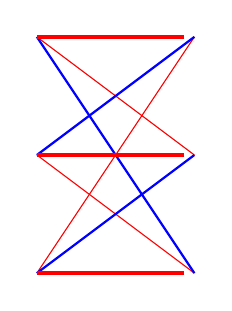
\begin{tikzpicture}[thick,scale=1]

\draw[color = red, thin] (-1,2.5)--(1,1);
\draw[color = red, thin] (-1,1)--(1,-.5);
\draw[color = red, thin] (-1,-0.5)--(1,2.5);
\draw[color = blue] (-1,2.5)--(1,-0.5);
\draw[color = blue] (-1,1)--(1,2.5);
\draw[color = blue] (-1,-0.5)--(1,1);

\draw (1, 2.5) node[]{}
	edge[color = red, ultra thick] (-1, 2.5);
\draw (-1, 2.5) node[]{};
\draw (1, 1) node[]{}
	edge[color = red, ultra thick] (-1, 1);
\draw (-1, 1) node[]{};
\draw (1, -0.5) node[]{}
	edge[color = red, ultra thick] (-1, -0.5);
\draw (-1, -0.5) node[]{};


\end{tikzpicture}
	\end{center}
	\caption{A red connected matching $M$ with an alternating cycle of length six.}
	\label{rb_cexp}
\end{figure}
This is very closely related to the problem of finding a connected matching in the graph of red edges.  In fact, a matching as described above with no alternating blue-red cycles would certainly be a connected matching.  As we proved in Chapter 4, for chordal bipartite graphs, the problems are equivalent.  However for general bipartite graphs it is stronger than the notion of a connected matching.  As we see in Figure \ref{rb_cexp}, a connected matching in red edges could permit alternating cycles longer than four edges.  

\section{General graphs}

Sometimes we may encounter a matching-type problem with only one type of object modeled by nodes.  In this case, we cannot assume that the appropriate graph model is bipartite.  The relation we wish to model with edges in the graph is assumed to be non-transitive, as otherwise the graph model degenerates into a collection of disconnected cliques.
	\subsection{Partnership assignments}
One type of ``assignment between equals'' we encounter in the real world is that of working partnerships.  In any organization, we can model individuals as vertices in a graph and use edges to represent some type of advantageous (non-transitive) working relationship.  By identifying a connected matching, we collect a set of possible partnerships wherein each pair of partners has the advantageous relationship and any two pairs $A$ and $B$ have an indvidual from pair $A$ that has the advantageous relationship with some individual from pair $B$,

Let us see how this might work in a high school mathematics classroom.  Suppose we model the students in the class as vertices. We are interested in the opportunities students have to work together outside of class, so we place an edge between vertices if the corresponding students share a study hall, lunch period, or live within a block of one another.  We want to assign a project to groups of two students each, and would like for the students to have time to work on the project outside of class.  Assigning groups so that each group corresponds to an edge in the graph we have constructed is a matching problem, and the result is a collection of pairs of students that have opportunities to work together outside of class.  

Now let's suppose that the content of each pair's assigned project is a piece of a larger class project.  In light of this, we would like to additionally require that each pair of two-student groups has a chance to share their findings and collaborate outside of class.  In order for this to happen, the matching must also be connected.  That is to say, in any two groups $A$ and $B$, there is a student from $A$ who shares a study hall, lunch period, or neighborhood with a student from $B$.  


		%Optimization with connected matchings
	\chapter{Future work}
In investigating connected matchings, many tangential problems arise that are quite interesting in their own right.  In this chapter, we discuss some of these, along with any progress made and possible areas of deeper investigation in the future.

\section{Characterizing the ``connected matching graph''}

The proximity partition induced by a graph $G$ can be thought of as the collection of \textit{distance-$k$ graphs} of $G$.
%
We may ask if there is a characterization of $\mathcal{H}_k$ where
%
\[\mathcal{H}_k = \{H :\: H \makebox{ is the distance-$k$ graph of some graph } G\}\]
%
In the case of $\mathcal{H}_2$, we can do so.
%
Let $A(G)$ denote the adjacency matrix of a graph $G$.  
%
In \cite{sqrtofgraph} Mukhopdhyay characterizes graphs that have a \textit{square root}, which is to say graphs $H$ such that for some graph $G$, $A(H) = A(G)^2$.
%  
This is equivalent to $H$ possesing an edge between any pair of vertices $u,v$ that satisfy $d_G(u,v) \leq 2$.  
%
\bthm{[Mudkhopdhyay] A connected graph $G$ with $n$ vertices $v_1, v_2, \ldots, v_n$ has a square root if and only if some set of $n$ complete subgraphs of $G$ whose union is $G$ can be labeled $C_1, C_2, \ldots, C_n$ so that, for all $i,j = 1, 2, \ldots, n$ the following conditions hold:
\begin{enumerate}
	\item $C_i$ contains $v_i$,
	\item $C_i$ contains $v_j$ if and only if $C_ij$ contains $v_i$.
\end{enumerate}}
\noindent An alternate definition of $\mathcal{H}_2$ is 
\[\mathcal{H}_2 = \{H : \: A(H) = A(G)^2-A(G)\}\] and we have the following characterization in the spirit of Mukhopdhyay's theorem.  
\bthm{A graph $G$ with $n$ vertices $v_1, v_2, \ldots , v_n$ is the distance 2 graph of some graph $H$ if and only if some set of $n$ subgraphs of $G$ whose union is $G$ can be labeled $C_1, C_2, \ldots, C_n$ so that 
\begin{enumerate}
	\item $v_a \notin C_a$ 
	\item For every pair of vertices $v_i, v_j \in C_k$, exactly one of the following holds:
	\begin{enumerate}
		\item $v_iv_j \in E(C_k)$ 
		\item If $v_i \in V(C_j)$, then $v_j \in V(C_i)$
		\item $v_i \in C_j$ and $v_j \in C_i$
	\end{enumerate}
	\item If $C_i \cap C_j \neq \emptyset$, then $v_i, v_j \in V(C_k)$ for some $k$.
\end{enumerate}}
The proof of this theorem rests on the same central realization as Mudkhopdhay's theorem, which is that the enumerated subgraphs correspond to the neighborhoods (closed neighborhoods in Mudkhopdhay's theorem, open ones in theorem REF) in the underlying graph.
\begin{proof}
Suppose we have a graph $G$ on vertices $v_1, v_2, \ldots, v_n$ and subgraphs $C_1, C_2, \ldots, C_n$ that satisfy the above hypotheses.  We construct a graph $H$ on the same vertex set by adding edges in two steps for each $C_i$.
\begin{description}
	\item[Step 1.] Add the complement of $C_i$.
	\item[Step 2.] Add all edges from $v_i$ to $C_i$.
\end{description}
	We claim that $G$ is now the distance 2 graph of $H$.  Suppose that $d_H(v_i, v_j) = 2$.  We want to show that $v_iv_j \in E(G)$.  Since $d_H(v_i,v_j) \leq 2$, there is some vertex $v_k$ so that $v_iv_k, v_jv_k \in E(H)$.  If both edges were added in step 2, then one of the following occurs
\begin{description}
	\item[Case 1.] $v_i, v_j \in C_k$
	\item[Case 2.] $v_k \in C_i$, $v_k \in C_j$
	\item[Case 3.] $v_k \in C_i, C_j$
\end{description}    
In case 1, distance 2 implies $v_iv_j \notin E(H)$. In particular, this edge was not added in step 2, so $v_i \notin C_j$ and $v_j \notin C_i$.  Condition 2 then implies that if $v_i, v_j \in C_k$ for some $C_k$, then $v_iv_j \in E(G)$.  In case 2, $V(C_i)$ and $V(C_j)$ intersect, implying (by condition 3) again that there is a $V(C_l)$ containing both $v_i$ and $v_j$.  In case 3, condition 4 requires that $v_i, v_j \in C_k$.  In any event, $v_iv_j \in E(G)$.

Now we may assume WLOG that $v_iv_k$ was added to $H$ in step 1.  Suppose $v_jv_k$ was added in step 2. Then either $v_k \in C_j$, implying $C_i \cap C_j \neq \emptyset$, or $v_j \in C_k$ implying $v_i, v_j \in C_k$.  The only remaining possibility is that both $v_iv_k$ and $v_jv_k$ were added in step 1.  Following from two applications of condition 2(b), both $v_i$ and $v_j$ are then in $V(C_k)$.  Sufficiency complete.

For the proof of necessity, we take a graph $H$ and show that its distance two graph $D_2(H)$ has a collection of subgraphs with the necessary properties.  For each vertex $v_i$, let $V(C_i) = N(v_i)$.  That condition 1 holds is immediate.  The vertices of any given $C_i$ are at most distance two apart.  Whenever there is a nonedge in a particular $C_i$ and 2(a) fails, the vertices must be adjacent in $H$, and condition 2(b) holds.  The symmetric property of the neighbor relation shows that conditions 3 and 4 hold as well.  Finally, all distance 2 edges occur between vertices with a common neighbor, so $\bigcup C_i = G$. 
\end{proof}

In a distance 2 graph, the enumerated subgraphs are actually the {\it complements} of the graphs induced by the open neighborhoods of the underlying graphs.  This allows us to characterize the distance 2 graphs of graphs with local characterizations.  The following is an example.
\bprop{If every enumerated subgraph $C_i$ of a distance 2 graph $H$ is triangle free, then it is the distance 2 graph of a claw-free graph.}
In the case of connected matchings, we are most interested in the distance 2 graphs of line graphs.  Unfortunately, line graphs do not have a local characterization.  The best local characterization that approximates them is the {\it locally co-bipartite} graphs.  A graph is locally co-bipartite if each open neighborhood induces a graph whose complement is bipartite.  Hence, the following is the best we have in the direction of characterizing the distance 2 graphs of line graphs.
\bprop{If every enumerated subgraph $C_i$ of a distance 2 graph $H$ is bipartite, then it is the distance 2 graph of a locally co-bipartite graph.}

\section{Tree Hypergraphs}

Chordal bipartite graphs, which figure heavily in chapter 4 of this dissertation, can be characterized as bipartite graph representations of a particular type of hypergraph.  
	%Future work
\backmatter

\addcontentsline{toc}{chapter}{REFERENCES}		


%\begin{bibsection}[Annotated Bibliography]\vspace{-\parskip} % This is the start of the bibliography. 
%	\begin{biblist}[\normalsize] % Replace the \bib entries with ones relevant to your problem.
							% The bulk of each entry can be copied and pasted from MathSciNet
							% ( http://www.ams.org/mathscinet/ ). When viewing the review of an
							% item you want to site, open the "Select alternative format" pull-down
							% and select AMSrefs.
							% Most likely, the only part you will need to change is the first parameter
							% after \bib. This is the internal name you use to cite the reference
							% with \cite. By default it will be the Mathematical Reviews number
							% (for example MR1375315). To make my life easier when I merge these all
							% into the summary document, please choose a name that begins with your
							% initials, followed by the number of problems you have submitted
							% (including this one).
							% For example, since this problem was submitted by Leonhard Euler and
							% since this is the first problem he is presenting, all citation names
							% begin with "le1". If this was his third problem, they would begin with
							% "le3".
%Z. Füredi, A. Gyárfás, G. Simonyi,  Connected matchings and Hadwiger's conjecture,  Combin. Probab. Comput., Problem Section, 14 (2005), 435--438.
%M. Kriesell, On seymour's strengthening of Hadwidger's conjecture for graphs with certain forbidden subgraphs 

%Mukhopadhyay, A. "The Square Root of a Graph." J. Combin. Th. 2, 290-295, 1967. 
\begin{thebibliography}{10}

\bib{PFTB}{book}{
   author={Aigner, Martin},
   author={Ziegler, G{\"u}nter M.},
   title={Proofs from The Book},
   edition={4},
   publisher={Springer-Verlag},
   place={Berlin},
   date={2010},
   pages={viii+274},
   isbn={978-3-642-00855-9},
   review={\MR{2569612 (2010m:00001)}},
   doi={10.1007/978-3-642-00856-6},
}
\bib{balogh}{article}{
   author={Balogh, J{\'o}zsef},
   author={Kostochka, Alexandr V.},
   title={Large minors in graphs with given independence number},
   journal={Discrete Math.},
   volume={311},
   date={2011},
   number={20},
   pages={2203--2215},
   issn={0012-365X},
   review={\MR{2825665 (2012i:05275)}},
   doi={10.1016/j.disc.2011.07.003},
}


\bib{Blas}{article}{
   author={Blasiak, Jonah},
   title={A special case of Hadwiger's conjecture},
   journal={J. Combin. Theory Ser. B},
   volume={97},
   date={2007},
   number={6},
   pages={1056--1073},
   issn={0095-8956},
   review={\MR{2354718 (2009a:05064)}},
   doi={10.1016/j.jctb.2007.04.003},
}

\bib{bohman}{article}{
   author={Bohman, Tom},
   title={The triangle-free process},
   journal={Adv. Math.},
   volume={221},
   date={2009},
   number={5},
   pages={1653--1677},
   issn={0001-8708},
   review={\MR{2522430 (2010h:05271)}},
   doi={10.1016/j.aim.2009.02.018},
}

\bib{hadwiger_aa}{article}{
   author={Bollob{\'a}s, B\'ela},
   author={Catlin, Paul},
   author={Erd{\H{o}}s, Paul A.},
   title={Hadwiger's conjecture is true for almost every graph},
   journal={European J. Combin.},
   volume={1},
   date={1980},
   number={3},
   pages={195--199},
   issn={0195-6698},
   review={\MR{593989 (82b:05107)}},
}



\bib{K_Cam_conn_match}{article}{
   author={Cameron, Kathie},
   title={Connected matchings},
   conference={
      title={Combinatorial optimization---Eureka, you shrink!},
   },
   book={
      series={Lecture Notes in Comput. Sci.},
      volume={2570},
      publisher={Springer},
      place={Berlin},
   },
   date={2003},
   pages={34--38},
   review={\MR{2163948 (2006c:90072)}},
   %doi={10.1007/3-540-36478-1_5},
}

\bib{indmatch}{article}{
   author={Cameron, Kathie},
   title={Induced matchings},
   note={First Montreal Conference on Combinatorics and Computer Science,
   1987},
   journal={Discrete Appl. Math.},
   volume={24},
   date={1989},
   number={1-3},
   pages={97--102},
   issn={0166-218X},
   review={\MR{1011265 (90g:05139)}},
   doi={10.1016/0166-218X(92)90275-F},
}
\bib{Catlin}{article}{
   author={Catlin, Paul A.},
   title={Haj\'os' graph-coloring conjecture: variations and
   counterexamples},
   journal={J. Combin. Theory Ser. B},
   volume={26},
   date={1979},
   number={2},
   pages={268--274},
   issn={0095-8956},
   review={\MR{532593 (81g:05057)}},
   doi={10.1016/0095-8956(79)90062-5},
}

\bib{spgt}{article}{
   author={Chudnovsky, Maria},
   author={Robertson, Neil},
   author={Seymour, Paul},
   author={Thomas, Robin},
   title={The strong perfect graph theorem},
   journal={Ann. of Math. (2)},
   volume={164},
   date={2006},
   number={1},
   pages={51--229},
   issn={0003-486X},
   review={\MR{2233847 (2007c:05091)}},
   doi={10.4007/annals.2006.164.51},
}



\bib{dirac}{article}{
   author={Dirac, Gabriel A.},
   title={A property of $4$-chromatic graphs and some remarks on critical
   graphs},
   journal={J. London Math. Soc.},
   volume={27},
   date={1952},
   pages={85--92},
   issn={0024-6107},
   review={\MR{0045371 (13,572f)}},
}



\bib{DandM}{article}{
   author={Duchet, Pierre},
   author={Meyniel, Henry},
   title={On Hadwiger's number and the stability number},
   conference={
      title={Graph theory},
      address={Cambridge},
      date={1981},
   },
   book={
      series={North-Holland Math. Stud.},
      volume={62},
      publisher={North-Holland},
      place={Amsterdam},
   },
   date={1982},
   pages={71--73},
   review={\MR{671905 (84h:05074)}},
}

\bib{edmonds}{article}{
   author={Edmonds, Jack},
   title={Paths, trees, and flowers},
   journal={Canad. J. Math.},
   volume={17},
   date={1965},
   pages={449--467},
   issn={0008-414X},
   review={\MR{0177907 (31 \#2165)}},
}

\bib{fox}{article}{
   author={Fox, Jacob},
   title={Complete minors and independence number},
   journal={SIAM J. Discrete Math.},
   volume={24},
   date={2010},
   number={4},
   pages={1313--1321},
   issn={0895-4801},
   review={\MR{2735925 (2011m:05293)}},
   doi={10.1137/090766814},
}

\bib{fradkin}{article}{
   author={Fradkin, Alexandra},
   title={Clique minors in claw-free graphs},
   journal={J. Combin. Theory Ser. B},
   volume={102},
   date={2012},
   number={1},
   pages={71--85},
   issn={0095-8956},
   review={\MR{2871768 (2012m:05332)}},
   doi={10.1016/j.jctb.2011.04.005},
}


\bib{GFS}{article}{
   author={F\"{u}redi, Zolt\'{a}n},
   author={Gy{\'a}rf{\'a}s, Andr{\'a}s},
   author={Simonyi, G\'{a}bor}
   title={Connected matchings and Hadwiger's conjecture},
   journal={Combin. Probab. Comput.},
   part={Problem Section},
   volume={14},
   date={2005},
   pages={435--438},
}

\bib{npcomplete}{book}{
   author={Garey, Michael R.},
   author={Johnson, David S.},
   title={Computers and intractability},
   note={A guide to the theory of NP-completeness;
   A Series of Books in the Mathematical Sciences},
   publisher={W. H. Freeman and Co.},
   place={San Francisco, Calif.},
   date={1979},
   pages={x+338},
   isbn={0-7167-1045-5},
   review={\MR{519066 (80g:68056)}},
}



\bib{Golumbic}{book}{
   author={Golumbic, Martin Charles},
   title={Algorithmic graph theory and perfect graphs},
   series={Annals of Discrete Mathematics},
   volume={57},
   edition={2},
   note={With a foreword by Claude Berge},
   publisher={Elsevier Science B.V.},
   place={Amsterdam},
   date={2004},
   pages={xxvi+314},
   isbn={0-444-51530-05},
   review={\MR{2063679 (2005e:05061)}},
}


\bib{Gol_Goss}{article}{
   author={Golumbic, Martin Charles},
   author={Goss, Clinton F.},
   title={Perfect elimination and chordal bipartite graphs},
   journal={J. Graph Theory},
   volume={2},
   date={1978},
   number={2},
   pages={155--163},
   issn={0364-9024},
   review={\MR{493395 (80d:05037)}},
   doi={10.1002/jgt.3190020209},
}

\bib{MR2249267}{article}{
   author={Gy{\'a}rf{\'a}s, Andr{\'a}s},
   author={Ruszink{\'o}, Mikl{\'o}s},
   author={S{\'a}rk{\"o}zy, G{\'a}bor N.},
   author={Szemer{\'e}di, Endre},
   title={One-sided coverings of colored complete bipartite graphs},
   conference={
      title={Topics in discrete mathematics},
   },
   book={
      series={Algorithms Combin.},
      volume={26},
      publisher={Springer},
      place={Berlin},
   },
   date={2006},
   pages={133--144},
   review={\MR{2249267 (2008c:05120)}},
   %doi={10.1007/3-540-33700-8_8},
}

\bib{hadwiger}{article}{
   author={Hadwiger, Hugo},
   title={\"Uber eine Klassifikation der Streckenkomplexe},
   language={German},
   journal={Vierteljschr. Naturforsch. Ges. Z\"urich},
   volume={88},
   date={1943},
   pages={133--142},
   review={\MR{0012237 (6,281c)}},
}

\bib{Kawa}{article}{
   author={Kawarabayashi, Ken-ichi},
   author={Plummer, Michael D.},
   author={Toft, Bjarne},
   title={Improvements of the theorem of Duchet and Meyniel on Hadwiger's
   conjecture},
   journal={J. Combin. Theory Ser. B},
   volume={95},
   date={2005},
   number={1},
   pages={152--167},
   issn={0095-8956},
   review={\MR{2156345 (2006b:05118)}},
   doi={10.1016/j.jctb.2005.04.001},
}


\bib{MR1844036}{article}{
   author={Kotlov, Andre{\u\i}},
   title={Matchings and Hadwiger's conjecture},
   note={Algebraic and topological methods in graph theory (Lake Bled,
   1999)},
   journal={Discrete Math.},
   volume={244},
   date={2002},
   number={1-3},
   pages={241--252},
   issn={0012-365X},
   review={\MR{1844036 (2002k:05087)}},
   doi={10.1016/S0012-365X(01)00087-5},
}

\bib{Kim}{article}{
   author={Kim, Jeong Han},
   title={The Ramsey number $R(3,t)$ has order of magnitude $t\sp 2/\log t$},
   journal={Random Structures Algorithms},
   volume={7},
   date={1995},
   number={3},
   pages={173--207},
   issn={1042-9832},
   review={\MR{1369063 (96m:05140)}},
   doi={10.1002/rsa.3240070302},
}

\bib{Kries_1}{article}{
   author={Kriesell, Matthias},
   title={On Seymour's strengthening of Hadwiger's conjecture for graphs with certain forbidden subgraphs},
   journal={Discrete Mathematics},
   %volume={},
   date={2010},
   pages={435--438},
}

\bib{Lehel}{article}{
   author={Lehel, Jen{\H{o}}},
   title={A characterization of totally balanced hypergraphs},
   journal={Discrete Math.},
   volume={57},
   date={1985},
   number={1-2},
   pages={59--65},
   issn={0012-365X},
   review={\MR{816048 (87f:05123)}},
   doi={10.1016/0012-365X(85)90156-6},
}

\bib{MR882610}{article}{
   author={Maffray, Frank},
   author={Meyniel, Henry},
   title={On a relationship between Hadwiger and stability numbers},
   journal={Discrete Math.},
   volume={64},
   date={1987},
   number={1},
   pages={39--42},
   issn={0012-365X},
   review={\MR{882610 (88g:05076)}},
   doi={10.1016/0012-365X(87)90238-X},
}

\bib{sqrtofgraph}{article}{
   author={Mukhopadhyay, Amar},
   title={The square root of a graph},
   journal={J. Combinatorial Theory},
   volume={2},
   date={1967},
   pages={290--295},
   review={\MR{0210616 (35 \#1502)}},
}



\bib{OST}{article}{
   author={Oron, Daniel},
   author={Steiner, George},
   author={Timkovsky, Vadim G.},
   title={The bipartite margin shop and maximum red matchings free of
   blue-red alternating cycles},
   journal={Discrete Optim.},
   volume={6},
   date={2009},
   number={3},
   pages={299--309},
   issn={1572-5286},
   review={\MR{2532467 (2010g:90052)}},
   doi={10.1016/j.disopt.2009.03.001},
}
\bib{pedersen}{article}{
   author={Pedersen, Anders Sune},
   author={Toft, Bjarne},
   title={A basic elementary extension of the Duchet-Meyniel theorem},
   journal={Discrete Math.},
   volume={310},
   date={2010},
   number={3},
   pages={480--488},
   issn={0012-365X},
   review={\MR{2564800 (2011c:05320)}},
   doi={10.1016/j.disc.2009.03.023},
}

\bib{PST}{article}{
   author={Plummer, Michael D.},
   author={Stiebitz, Michael},
   author={Toft, Bjarne},
   title={On a special case of Hadwiger's conjecture},
   journal={Discuss. Math. Graph Theory},
   volume={23},
   date={2003},
   number={2},
   pages={333--363},
   issn={1234-3099},
   review={\MR{2070161 (2005e:05055)}},
}

\bib{ramsey}{article}{
   author={Ramsey, Frank P.},
   title={On a Problem of Formal Logic},
   journal={Proc. London Math. Soc.},
   volume={S2-30},
   number={1},
   pages={264},
   issn={0024-6115},
   review={\MR{1576401}},
   doi={10.1112/plms/s2-30.1.264},
}


\bib{HCK6}{article}{
   author={Robertson, Neil},
   author={Seymour, Paul},
   author={Thomas, Robin},
   title={Hadwiger's conjecture for $K\sb 6$-free graphs},
   journal={Combinatorica},
   volume={13},
   date={1993},
   number={3},
   pages={279--361},
   issn={0209-9683},
   review={\MR{1238823 (94i:05037)}},
   doi={10.1007/BF01202354},
}


\bib{toft_survey}{article}{
   author={Toft, Bjarne},
   title={A survey of Hadwiger's conjecture},
   note={Surveys in graph theory (San Francisco, CA, 1995)},
   journal={Congr. Numer.},
   volume={115},
   date={1996},
   pages={249--283},
   issn={0384-9864},
   review={\MR{1411244 (97i:05048)}},
}

\bib{turan}{article}{
   author={Tur{\'a}n, Paul},
   title={Eine Extremalaufgabe aus der Graphentheorie},
   language={Hungarian, with German summary},
   journal={Mat. Fiz. Lapok},
   volume={48},
   date={1941},
   pages={436--452},
   review={\MR{0018405 (8,284j)}},
}
\bib{dwest}{book}{
   author={West, Douglas B.},
   title={Introduction to graph theory},
   publisher={Prentice Hall Inc.},
   place={Upper Saddle River, NJ},
   date={1996},
   pages={xvi+512},
   isbn={0-13-227828-6},
   review={\MR{1367739 (96i:05001)}},
}




































\end{thebibliography}
\nocite{*}
		%bibliography
	
\printindex\addcontentsline{toc}{chapter}{INDEX}
\setstretch{1}
\pagebreak
~\vspace{0.5 in}
\begin{center}

CURRICULUM VITAE

\end{center}

\vskip 0.25 cm
\noindent NAME: \tabto{3.5 cm} Christopher Caraganis\\\vskip 0.25 cm
\noindent ADDRESS: \tabto{3.5 cm} 3913 Southern Pkwy\\
\tabto{3.5 cm} Louisville, KY  40214\\
\vskip 0.25 cm
\noindent DOB: \tabto{3.5 cm} Louisville, KY - August 4, 1980\\

\vskip 0.25 cm \noindent EDUCATION\\
\& TRAINING \tabto{4.5 cm} B.S., Mathematics\\
\tabto{4.5 cm} University of Louisville\\
\tabto{4.5 cm} 2004-2007\\
\vskip 0.25 cm
\tabto{4.5 cm} M.A., Mathematics\\
\tabto{4.5 cm} University of Louisville\\
\tabto{4.5 cm} 2007-2009\\
\vskip 0.25 cm\tabto{4.5 cm} Ph.D., Mathematics\\
\tabto{4.5 cm} Univerity of Louisville\\
\tabto{4.5 cm} 2009-2012\\
\vskip 0.25 cm\noindent AWARDS: \tabto{3.5 cm} Logistics and Distribution Institute\\
\tabto{3.5 cm} Graduate Research Assistantship\\
\tabto{3.5 cm} 2010\\
\vskip 0.25 cm
\tabto{3.5 cm} College of Arts and Sciences Outstanding Graduate Award\\
\tabto{3.5 cm} 2009\\
\vskip 0.25 cm
\tabto{3.5 cm} Graduate Dean's Citation\\
\tabto{3.5 cm} 2009\\

\addcontentsline{toc}{chapter}{CURRICULUM VITAE}
	

\end{document}
